%_____________________________________________________________________________
%=============================================================================
% main.tex v8 (31-05-2015) \ldots dibuat oleh Lionov - Informatika FTIS UNPAR
% 
% Ini adalah file utama (main.tex), berisi perintah-perintah yang khusus 
% dibuat untuk template ini
%
% 			JANGAN MENGUBAH APAPUN DI DALAM FILE INI,
%			KECUALI ANDA TAHU APA YANG ANDA LAKUKAN !!!
%
% Jika ada tambahan perintah, dapat anda tuliskan di tempat yang telah disediakan 
% di baris 310 pada file ini
% Jika daftar tabel tidak digunakan, anda harus menghapus (beri komentar) secara
% manual di baris 485
%
% Bug, kritik, saran: silahkan kirimkan via email ke lionov@unpar.ac.id
%
% Perubahan pada versi 8 (31-05-2015):
%	- penambahan default data untuk beberapa keterangan dan digunakan sebagai 
%	  template dengan tanda << & >> . Data yang diubah defaultnya adalah: nama skripsi
%	  nama prodi, beserta bahasa inggrisnya.
%   - Keywords dan kata kunci di abstrak ditambahkan noindent + perbaikan lainnya
%   - Perbaikan untuk halaman tidak kosong tanpa nomor halaman romawi
%
% Perubahan pada versi sebelumnya :
%	versi 7 (27-05-2014)
%	- penambahan perintah \raggedbottom untuk menghilangkan area kosong akibat 
%	  penempatan gambar yang tidak sempurna
%	versi 6 (10-11-2013)
%	- perbaikan pada abstract dengan paragraf lebih dari satu: perbaikan vertical spacing
%	- perbaikan pada tampilan bab dan lampiran: tidak perlu menuliskan apapun untuk 
%	  menampilkan semuanya (di data.tex) atau -1 jika tidak ada lampiran
%	- halaman bernomor genap untuk halaman romawi sudah dimunculkan
%	- Kurikulum 2013 : perubahan nama buku skripsi 
%	versi 5 (21-10-2012)
%	- halaman terakhir setiap bab tidak ada headernya jika kosong
%	versi 4 (06-08-2012)
% 	- penggabungan main.tex, depan.tex dan setup.tex menjadi main.tex
% 	- menambahkan keterangan di lampiran untuk kode program 
% 	- ukuran font dapat diubah langsung di tiap lampiran
% 	versi 3 (09-07-2012): 
%	- Tidak ada di file ini
% 	versi 2 :
% 	- "Daftar Referensi" tidak perlu diubah secara manual (tidak perlu mengubah file bahasai.ldf)
% 	- Bahasa Indonesia dari abstract adalah abstrak (secara otomatis), bukan ringkasan
% 	- Spasi pada buku dokumen final adalah onehalfspacing
%
% to do : - hilangkan secara otomatis daftar tabel/gambar jika tidak digunakan
%         - (IT) aturan penulisan algoritma untuk IT (pakai algo.sty ?)
%=============================================================================

%=============================================================================
% setup.tex v2 (08-07-2012)
% Perubahan pada versi 2:
% - Menambahkan perintah untuk judulINA dan judulENG
% - Menghapus \usepackage{microtype}, yang pada beberapa kasus menjadi masalah
%=============================================================================
% depan.tex v2 (09-07-2012)
% Perubahan pada versi 2:
% - Menambahkan halaman depan dalam bahasa inggris
%=============================================================================

%setup.tex
\documentclass[11pt,a4paper,twoside,openright,notitlepage]{report} 

\usepackage[bahasa]{babel} %bahasa indonesia
\usepackage[T1]{fontenc}  %encoding
% \usepackage{mathptmx}
% \usepackage{venturisold}
% \usepackage{helvet}
% \usepackage{fouriernc} 
\usepackage{abstract} %manipulasi abstract
\usepackage{chappg} % format daftar isi 
\usepackage{color} %warna
\usepackage{etoolbox} %untuk programming if-then
\usepackage{fancyhdr} %format header & footer
\usepackage{float} %penempatan gambar di tempat yg seharusnya
\usepackage[inner=2.5cm,outer=2cm,top=2.5cm,bottom=2.5cm]{geometry} %margin
\usepackage{graphicx} %gambar
\usepackage{listings} %source code
\usepackage{lscape} %landscape untuk source code
\usepackage{multicol} %multiple column
\usepackage{ifthen} % if then
\usepackage[pagewise]{lineno} %line numbering
\usepackage{lipsum} % untuk testing
\usepackage{titlesec} %judul header
\usepackage{tocbibind} %daftar isi, gambar, tabel dll
\usepackage{tocloft} % format daftar isi 
\usepackage{setspace} %line spacing
\usepackage{xstring} %manipulasi string
\usepackage[plainpages=false,pdfpagelabels,unicode]{hyperref} %\autoref, \phantomsection & link 
\usepackage{emptypage}

\let\abstractname\Abstrak

\titleformat{\chapter}[display] {\Large\bfseries\centering}{\MakeUppercase{\chaptertitlename} \thechapter}{15pt}{\Large\MakeUppercase}

\renewcommand{\cftchapfont}{\scshape \bfseries}

\renewcommand{\cfttoctitlefont}{\hfill\Large\bfseries\MakeUppercase}
\renewcommand{\cftaftertoctitle}{\hfill}
\renewcommand{\cftloftitlefont}{\hfill\Large\bfseries\MakeUppercase}
\renewcommand{\cftafterloftitle}{\hfill}
\renewcommand{\cftlottitlefont}{\hfill\Large\bfseries\MakeUppercase}
\renewcommand{\cftafterlottitle}{\hfill}

% Tidak perlu ada kata "Bab", "Gambar" atau "Tabel" di daftar 
% \renewcommand{\cftchappresnum}{{\bf \scshape Bab} } 
% \renewcommand{\cftchapnumwidth}{1.5cm}
% \renewcommand{\cftfigpresnum}{{Gambar\ }} 
% \renewcommand{\cftfignumwidth}{2.5cm}
% \renewcommand{\cfttabpresnum}{{Tabel\ }} 
% \renewcommand{\cfttabnumwidth}{2cm}

\newcommand{\apptoc}{
	% Hapus kata "Lampiran" dari daftar isi
	%\addtocontents{toc}{\protect\renewcommand{\protect\cftchappresnum}{\bf \scshape Lampiran\  }}%
	%\addtocontents{toc}{\protect\renewcommand{\protect\cftchapnumwidth}{2.75cm}}
	\addtocontents{toc}{\protect\renewcommand{\protect\cftchappresnum}{\bf \scshape}}%	

}

\newcommand{\vnama}{Jane Doe}
\newcommand{\vlnama}{John Doe}
\newcommand{\vnpm}{1992700001}
\newcommand{\vprodiINA}{SAINS}
\newcommand{\vprodiENG}{SCIENCE}
\newcommand{\vstaINA}{UJIAN}
\newcommand{\vstaENG}{EXAM}
%\newcommand{\vjudul}{Judul Skripsi/Tugas Akhir}
\newcommand{\vpembu}{Plato}
\newcommand{\vpembs}{Euclid}
\newcommand{\vpengi}{Plato}
\newcommand{\vpengii}{Euclid}
\newcommand{\vtanggal}{1}
\newcommand{\vbulan}{Januari}
\newcommand{\vtahun}{1970}
\newcommand{\vmode}{final}
\newcommand{\vspacing}{double}
\newcommand{\vlineno}{yes}
\newcommand{\vkunciina}{Skripsi, Tugas Akhir}
\newcommand{\vkuncieng}{Undergraduate Thesis, Final Project}
\newcommand{\vkajur}{Jack Doe}
\newcommand{\vkajurmat}{Jack Doe}
\newcommand{\vkajurfis}{Jack Doe}
\newcommand{\vkajurtif}{Jack Doe}

\newcommand{\namanpm}[2]{
	\renewcommand{\vstaINA}{<<SKRIPSI/TUGAS AKHIR>>}
	\renewcommand{\vprodiINA}{<<MATEMATIKA/FISIKA/TEKNIK INFORMATIKA>>}
	\renewcommand{\vstaENG}{<<FINAL PROJECT/UNDERGRADUATE THESIS>>}
	\renewcommand{\vprodiENG}{<<MATHEMATICS/PHYSICS/INFORMATICS>>}
	\renewcommand{\vnama}{\uppercase{#1}} \renewcommand{\vlnama}{#1} \hypersetup{pdfauthor={#2 - #1}}
	\renewcommand{\vnpm}{#2} \hypersetup{pdfcreator={#2}} \StrChar{\vnpm}{6}[\vprodiN]
	\ifdefstring{\vprodiN}{1}{
		\renewcommand{\vprodiINA}{MATEMATIKA} \renewcommand{\vprodiENG}{MATHEMATICS} 
		\renewcommand{\vstaINA}{SKRIPSI} \renewcommand{\vstaENG}{FINAL PROJECT} \renewcommand{\vkajur}{\vkajurmat}}{}
	\ifdefstring{\vprodiN}{2}{
		\renewcommand{\vprodiINA}{FISIKA} \renewcommand{\vprodiENG}{PHYSICS} 
		\renewcommand{\vstaINA}{TUGAS AKHIR} \renewcommand{\vstaENG}{FINAL PROJECT} \renewcommand{\vkajur}{\vkajurfis}}{}
	\ifdefstring{\vprodiN}{3}{
		\renewcommand{\vprodiINA}{TEKNIK INFORMATIKA} \renewcommand{\vprodiENG}{INFORMATICS} 
		\renewcommand{\vstaINA}{CONTOH SKRIPSI} \renewcommand{\vstaENG}{UNDERGRADUATE THESIS EXAMPLE} \renewcommand{\vkajur}{\vkajurtif}}{}}

%\newcommand{\judul}[1]{\renewcommand{\vjudul}{\uppercase{#1}}\hypersetup{pdftitle={#1}, pdfsubject={#1}}}
\newcommand{\pembimbing}[2]{\renewcommand{\vpembu}{#1}\renewcommand{\vpembs}{#2}}
\newcommand{\penguji}[2]{\renewcommand{\vpengi}{#1}\renewcommand{\vpengii}{#2}}
\newcommand{\kajur}[3]{\renewcommand{\vkajurmat}{#1}\renewcommand{\vkajurfis}{#2}\renewcommand{\vkajurtif}{#3}}
\renewcommand{\vbulan}{<<bulan>>}
\newcommand{\tanggal}[3]{\renewcommand{\vtanggal}{#1}\renewcommand{\vtahun}{#3}
	\newcommand{\vcbulan}{#2}
	\ifdefstring{\vcbulan}{1}{\renewcommand{\vbulan}{Januari}}{}
	\ifdefstring{\vcbulan}{2}{\renewcommand{\vbulan}{Februari}}{}
	\ifdefstring{\vcbulan}{3}{\renewcommand{\vbulan}{Maret}}{}
	\ifdefstring{\vcbulan}{4}{\renewcommand{\vbulan}{April}}{}
	\ifdefstring{\vcbulan}{5}{\renewcommand{\vbulan}{Mei}}{}
	\ifdefstring{\vcbulan}{6}{\renewcommand{\vbulan}{Juni}}{}
	\ifdefstring{\vcbulan}{7}{\renewcommand{\vbulan}{Juli}}{}
	\ifdefstring{\vcbulan}{8}{\renewcommand{\vbulan}{Agustus}}{}
	\ifdefstring{\vcbulan}{9}{\renewcommand{\vbulan}{September}}{}
	\ifdefstring{\vcbulan}{10}{\renewcommand{\vbulan}{Oktober}}{}
	\ifdefstring{\vcbulan}{11}{\renewcommand{\vbulan}{November}}{}
	\ifdefstring{\vcbulan}{12}{\renewcommand{\vbulan}{Desember}}{}	
}

\newcommand{\judulINA}[1]{\newcommand{\vjudulINA}{\uppercase{#1}}\hypersetup{pdftitle={#1},pdfsubject={#1}}}
\newcommand{\judulENG}[1]{\newcommand{\vjudulENG}{\uppercase{#1}}\hypersetup{pdftitle={#1},pdfsubject={#1}}}
\newcommand{\abstrakINA}[1]{\newcommand{\vabstrakina}{#1}}
\newcommand{\abstrakENG}[1]{\newcommand{\vabstrakeng}{#1}}
\newcommand{\kunciINA}[1]{\renewcommand{\vkunciina}{#1} \hypersetup{pdfkeywords={#1}}}
\newcommand{\kunciENG}[1]{\renewcommand{\vkuncieng}{#1}}
\newcommand{\untuk}[1]{\newcommand{\vuntuk}{#1}}
\newcommand{\prakata}[1]{\newcommand{\vprakata}{#1}}
\newcommand{\mode}[1]{\renewcommand{\vmode}{#1}}
\newcommand{\linespacing}[1]{\renewcommand{\vspacing}{#1}}
\newcommand{\linenumber}[1]{\renewcommand{\vlineno}{#1}}

\newcommand{\bab}[1]{\newcommand{\vbab}{#1}}
\newcommand{\lampiran}[1]{\renewcommand{\vlmp}{#1}}

\newcommand{\vpilbab}{0}
\newcommand{\vbaba}{0}\newcommand{\vbabb}{0}\newcommand{\vbabc}{0}
\newcommand{\vbabd}{0}\newcommand{\vbabe}{0}\newcommand{\vbabf}{0}
\newcommand{\vbabg}{0}\newcommand{\vbabh}{0}\newcommand{\vbabi}{0}
\newcommand{\vpillmp}{0}
\newcommand{\vlmpa}{0}\newcommand{\vlmpb}{0}\newcommand{\vlmpc}{0}
\newcommand{\vlmpd}{0}\newcommand{\vlmpe}{0}\newcommand{\vlmpf}{0}
\newcommand{\vlmpg}{0}\newcommand{\vlmph}{0}\newcommand{\vlmpi}{0}
\newcommand{\vlmp}{x}

%	\ifdefempty{#1}{\bab{1,2,3,4,5,6,7,8,9} \tampilbab{\vbab}}{
\newcommand{\tampilbab}[1]{
	\ifdefempty{#1}{
		\renewcommand{\vbaba}{1}\renewcommand{\vbabb}{1}\renewcommand{\vbabc}{1}
		\renewcommand{\vbabd}{1}\renewcommand{\vbabe}{1}\renewcommand{\vbabf}{1}
		\renewcommand{\vbabg}{1}\renewcommand{\vbabh}{1}\renewcommand{\vbabi}{1}}{
	\renewcommand{\do}[1]{
		\renewcommand{\vpilbab}{##1}
		\ifdefstring{\vpilbab}{1}{\renewcommand{\vbaba}{1}}{}
		\ifdefstring{\vpilbab}{2}{\renewcommand{\vbabb}{1}}{}
		\ifdefstring{\vpilbab}{3}{\renewcommand{\vbabc}{1}}{}
		\ifdefstring{\vpilbab}{4}{\renewcommand{\vbabd}{1}}{}
		\ifdefstring{\vpilbab}{5}{\renewcommand{\vbabe}{1}}{}
		\ifdefstring{\vpilbab}{6}{\renewcommand{\vbabf}{1}}{}
		\ifdefstring{\vpilbab}{7}{\renewcommand{\vbabg}{1}}{}
		\ifdefstring{\vpilbab}{8}{\renewcommand{\vbabh}{1}}{}
		\ifdefstring{\vpilbab}{9}{\renewcommand{\vbabi}{1}}{}
	}
	\expandafter\docsvlist\expandafter{#1}
	}
}

\newcommand{\tampillmp}[1]{
	\ifdefempty{#1}{
		\renewcommand{\vlmpa}{1}\renewcommand{\vlmpb}{1}\renewcommand{\vlmpc}{1}
		\renewcommand{\vlmpd}{1}\renewcommand{\vlmpe}{1}\renewcommand{\vlmpf}{1}
		\renewcommand{\vlmpg}{1}\renewcommand{\vlmph}{1}\renewcommand{\vlmpi}{1}}{
	\ifdefstring{#1}{-1}{ }{
		\renewcommand{\do}[1]{ 
			\renewcommand{\vpillmp}{##1}
			\ifdefstring{\vpillmp}{A}{\renewcommand{\vlmpa}{1}}{}
			\ifdefstring{\vpillmp}{B}{\renewcommand{\vlmpb}{1}}{}
			\ifdefstring{\vpillmp}{C}{\renewcommand{\vlmpc}{1}}{}
			\ifdefstring{\vpillmp}{D}{\renewcommand{\vlmpd}{1}}{}
			\ifdefstring{\vpillmp}{E}{\renewcommand{\vlmpe}{1}}{}
			\ifdefstring{\vpillmp}{F}{\renewcommand{\vlmpf}{1}}{}
			\ifdefstring{\vpillmp}{G}{\renewcommand{\vlmpg}{1}}{}
			\ifdefstring{\vpillmp}{H}{\renewcommand{\vlmph}{1}}{}
			\ifdefstring{\vpillmp}{I}{\renewcommand{\vlmpi}{1}}{}}
		}
	\expandafter\docsvlist\expandafter{#1}
	}
}

\newcommand{\appspacing}{
	\ifdefstring{\vspacing}{single}{\singlespacing}{}
	\ifdefstring{\vspacing}{onehalf}{\onehalfspacing}{}
	\ifdefstring{\vspacing}{double}{\doublespacing}{}
	\ifdefstring{\vmode}{final}{\onehalfspacing}{}
}

\newcommand{\appline}{
	\ifdefstring{\vmode}{final}{\renewcommand{\vlineno}{no}}{}
	\ifdefstring{\vlineno}{yes}{\linenumbers \def\linenumberfont{\normalfont\tiny\sffamily}}{}
	\ifdefstring{\vlineno}{no}{\lstset{numbers=left, stepnumber=1, numbersep=5pt}}{}
	
}

\newcommand{\appmargin}{
	\ifdefstring{\vmode}{final}{}{\newgeometry{inner=3cm,outer=2.75cm,top=2cm,bottom=2cm}}
}

\renewcommand{\abstractnamefont}{\bf \MakeUppercase}

\makeatletter
\def\headrule{{%
  \if@fancyplain\let\headrulewidth\plainheadrulewidth\fi
  \hrule\@height\footrulewidth\@width\headwidth\vskip2pt%
  \hrule\@height\headrulewidth\@width\headwidth\vskip-\headrulewidth\vskip-4pt
}}
\def\footrule{}

\def\cleardoublepage{
	\clearpage
	\if@twoside \ifodd\c@page
	\else
		\hbox{}
		\vspace{\fill}
		\thispagestyle{empty}
		\newpage
	\if@twocolumn\hbox{}\newpage\fi\fi\fi}
\makeatother

\renewcommand{\headrulewidth}{1.25pt}
\renewcommand{\footrulewidth}{0.25pt}

\setlength{\headheight}{15pt}
\fancyhead[LE,RO]{\thepage}
\fancyhead[RE]{\small{\textsc{\nouppercase{\leftmark}}}}
\fancyhead[LO]{\small{\textsc{\nouppercase{\rightmark}}}}
\fancyfoot{}

\hypersetup{unicode=true,colorlinks=true,linkcolor=blue,citecolor=green,filecolor=magenta, urlcolor=cyan}

\lstset{basicstyle=\tiny, commentstyle=\color{blue}}
\lstset{frame=leftline, tabsize=4, breaklines=true}

%=============================================================================

%tambahkan perintah yang anda butuhkan di sini :

%=============================================================================
%end setup.tex

%_____________________________________________________________________________
%=============================================================================
% data.tex v6 (13-04-2015) \ldots dibuat oleh Lionov - Informatika FTIS UNPAR
%
% Perubahan pada versi 6 (13-04-2015)
% - Perubahan untuk data-data ``template" menjadi lebih generik dan menggunakan
%	tanda << dan >>
%
% Perubahan pada versi sebelumnya
% 	versi 5 (10-11-2013)
% 	- Perbaikan pada memasukkan bab : tidak perlu menuliskan apapun untuk 
%	  memasukkan seluruh bab (bagian V)
% 	- Perbaikan pada memasukkan lampiran : tidak perlu menuliskan apapun untuk
%	  memasukkan seluruh lampiran atau -1 jika tidak memasukkan apapun
%	versi 4 (21-10-2012)
%	- Data dosen dipindah ke dosen.tex agar jika ada perubahan/update data dosen
%   mahasiswa tidak perlu mengubah data.tex
%	- Perubahan pada keterangan dosen	
% 	versi 3 (06-08-2012)
% 	- Perubahan pada beberapa keterangan 
% 	versi 2 (09-07-2012):
% 	- Menambahkan data judul dalam bahasa inggris
% 	- Membuat bagian khusus untuk judul (bagian VIII)
% 	- Perbaikan pada gelar dosen
%_____________________________________________________________________________
%=============================================================================
% 								BAGIAN -
%=============================================================================
% Ini adalah file data (data.tex)
% Masukkan ke dalam file ini, data-data yang diperlukan oleh template ini
% Cara memasukkan data dijelaskan di setiap bagian
% Data yang WAJIB dan HARUS diisi dengan baik dan benar adalah SELURUHNYA !!
% Hilangkan tanda << dan >> jika anda menemukannya
%=============================================================================
%_____________________________________________________________________________
%=============================================================================
% 								BAGIAN I
%=============================================================================
% Tambahkan package2 lain yang anda butuhkan di sini
%=============================================================================
\usepackage{booktabs}
\usepackage[table]{xcolor}
\usepackage{longtable}
\usepackage{amsmath}
%=============================================================================

%_____________________________________________________________________________
%=============================================================================
% 								BAGIAN II
%=============================================================================
% Mode dokumen: menetukan halaman depan dari dokumen, apakah harus mengandung 
% prakata/pernyataan/abstrak dll (termasuk daftar gambar/tabel/isi) ?
% - kosong : tidak ada halaman depan sama sekali (untuk dokumen yang 
%            dipergunakan pada proses bimbingan)
% - cover : cover saja tanpa daftar isi, gambar dan tabel
% - sidang : cover, daftar isi, gambar, tabel (IT: UTS-UAS Seminar 
%			 dan UTS TA)
% - sidang_akhir : mode sidang + abstrak + abstract
% - final : seluruh halaman awal dokumen (untuk cetak final)
% Jika tidak ingin mencetak daftar tabel/gambar (misalkan karena tidak ada 
% isinya), edit manual di baris 439 dan 440 pada file main.tex
%=============================================================================
% \mode{kosong}
% \mode{cover}
% \mode{sidang}
%\mode{sidang_akhir}
\mode{final} 
%=============================================================================

%_____________________________________________________________________________
%=============================================================================
% 								BAGIAN III
%=============================================================================
% Line numbering: penomoran setiap baris, otomatis di-reset setiap berganti
% halaman
% - yes: setiap baris diberi nomor
% - no : baris tidak diberi nomor, otomatis untuk mode final
%=============================================================================
\linenumber{yes}
%=============================================================================

%_____________________________________________________________________________
%=============================================================================
% 								BAGIAN IV
%=============================================================================
% Linespacing: jarak antara baris 
% - single: opsi yang disediakan untuk bimbingan, jika pembimbing tidak
%            keberatan (untuk menghemat kertas)
% - onehalf: default dan wajib (dan otomatis) jika ingin mencetak dokumen
%            final/untuk sidang.
% - double : jarak yang lebih lebar lagi, jika pembimbing berniat memberi 
%            catatan yg banyak di antara baris (dianjurkan untuk bimbingan)
%=============================================================================
\linespacing{single}
% \linespacing{onehalf}
%\linespacing{double}
%=============================================================================

%_____________________________________________________________________________
%=============================================================================
% 								BAGIAN V
%=============================================================================
% Bab yang akan dicetak: isi dengan angka 1,2,3 s.d 9, sehingga bisa digunakan
% untuk mencetak hanya 1 atau beberapa bab saja
% Jika lebih dari 1 bab, pisahkan dengan ',', bab akan dicetak terurut sesuai 
% urutan bab.
% Untuk mencetak seluruh bab, kosongkan parameter (i.e. \bab{ })  
% Catatan: Jika ingin menambahkan bab ke-10 dan seterusnya, harus dilakukan 
% secara manual
%=============================================================================
\bab{ }
%=============================================================================

%_____________________________________________________________________________
%=============================================================================
% 								BAGIAN VI
%=============================================================================
% Lampiran yang akan dicetak: isi dengan huruf A,B,C s.d I, sehingga bisa 
% digunakan untuk mencetak hanya 1 atau beberapa lampiran saja
% Jika lebih dari 1 lampiran, pisahkan dengan ',', lampiran akan dicetak 
% terurut sesuai urutan lampiran
% Jika tidak ingin mencetak lampiran apapun, isi dengan -1 (i.e. \lampiran{-1})
% Untuk mencetak seluruh mapiran, kosongkan parameter (i.e. \lampiran{ })  
% Catatan: Jika ingin menambahkan lampiran ke-J dan seterusnya, harus 
% dilakukan secara manual
%=============================================================================
\lampiran{ }
%=============================================================================

%_____________________________________________________________________________
%=============================================================================
% 								BAGIAN VII
%=============================================================================
% Data diri dan skripsi/tugas akhir
% - namanpm: Nama dan NPM anda, penggunaan huruf besar untuk nama harus benar
%			 dan gunakan 10 digit npm UNPAR, PASTIKAN BAHWA BENAR !!!
%			 (e.g. \namanpm{Jane Doe}{1992710001}
% - judul : Dalam bahasa Indonesia, perhatikan penggunaan huruf besar, judul
%			tidak menggunakan huruf besar seluruhnya !!! 
% - tanggal : isi dengan {tangga}{bulan}{tahun} dalam angka numerik, jangan 
%			  menuliskan kata (e.g. AGUSTUS) dalam isian bulan
%			  Tanggal ini adalah tanggal dimana anda akan melaksanakan sidang 
%			  ujian akhir skripsi/tugas akhir
% - pembimbing: isi dengan pembimbing anda, lihat daftar dosen di file dosen.tex
%				jika pembimbing hanya 1, kosongkan parameter kedua 
%				(e.g. \pembimbing{\JND}{  } ) , \JND adalah kode dosen
% - penguji : isi dengan para penguji anda, lihat daftar dosen di file dosen.tex
%				(e.g. \penguji{\JHD}{\JCD} ) , \JND dan \JCD adalah kode dosen
%
%=============================================================================
\namanpm{Pascal Alfadian Nugroho}{2003730013}	%hilangkan tanda << & >>
\tanggal{19}{3}{2015}			%hilangkan tanda << & >>
\pembimbing{\LNV}{}     %Lihat singkatan pembimbing anda di file dosen.tex
%Lihat singkatan pembimbing anda di file dosen.tex, hilangkan tanda << & >>
\penguji{\TAB}{\CEN} 		%Lihat singkatan penguji anda di file dosen.tex
%Lihat singkatan penguji anda di file dosen.tex, hilangkan tanda << & >>
%=============================================================================

%_____________________________________________________________________________
%=============================================================================
% 								BAGIAN VIII
%=============================================================================
% Judul dan title : judul bhs indonesia dan inggris
% - judulINA: judul dalam bahasa indonesia
% - judulENG: title in english
% PERHATIAN: - langsung mulai setelah '{' awal, jangan mulai menulis di baris 
%			   bawahnya
%			 - Gunakan \texorpdfstring{\\}{} untuk pindah ke baris baru
%			 - Judul TIDAK ditulis dengan menggunakan huruf besar seluruhnya !!
%			 - Gunakan perintah \texorpdfstring{\\}{} untuk baris baru
%=============================================================================

\judulINA{Integrasi Situs Navigasi dengan Situs \textit{Crowdsourcing} Rute Angkot}

\judulENG{Integration of \textit{Angkot} Navigation and Route Crowdsourcing Website}

%_____________________________________________________________________________
%=============================================================================
% 								BAGIAN IX
%=============================================================================
% Abstrak dan abstract : abstrak bhs indonesia dan inggris
% - abstrakINA: abstrak bahasa indonesia
% - abstrakENG: abstract in english
% PERHATIAN: langsung mulai setelah '{' awal, jangan mulai menulis di baris 
%			 bawahnya
%=============================================================================

\abstrakINA{Penelitian ini mengintegrasikan situs navigasi rute angkot
	\url{http://kiri.travel} dengan situs \textit{crowdsourcing} rute angkot 
	\url{https://angkot.web.id}, di mana pengguna dapat berkontribusi memperbaiki
	rute angkot yang salah. Integrasi yang dimaksud adalah sinkronisasi data secara
	berkala dan otomatis, sehingga hasil navigasi yang diberikan mendekati ketepatan
	sesuai di lapangan.

	TODO Sisa abstrak akan dilengkapi saat penelitian berakhir.
}

\abstrakENG{This research integrates \textit{angkot} (public bus) navigation website
	\url{http://kiri.travel} with \textit{angkot} route crowdsourcing website,
	where public user can contribute by fixing erroneus \textit{angkot} routes.
	The aforementioned integration is defined as automatic synchronization of
	both parties' data, such that the result accuracy of navigation is close to
	what found on the field.

	TODO The rest of abstract will be completed at end of research.
} 

%=============================================================================

%_____________________________________________________________________________
%=============================================================================
% 								BAGIAN X
%=============================================================================
% Kata-kata kunci dan keywords : diletakkan di bawah abstrak (ina dan eng)
% - kunciINA: kata-kata kunci dalam bahasa indonesia
% - kunciENG: keywords in english
%=============================================================================
\kunciINA{\textit{crowdsourcing}, angkot, rute, navigasi, \textit{REST}, \textit{JSON}}

\kunciENG{crowdsourcing, route, navigation, REST, JSON}
%=============================================================================

%_____________________________________________________________________________
%=============================================================================
% 								BAGIAN XI
%=============================================================================
% Persembahan : kepada siapa anda mempersembahkan skripsi ini ...
%=============================================================================
\untuk{
	Dipersembahkan untuk seluruh warga Indonesia yang selalu setia menggunakan transportasi umum dan mahasiswa FTIS UNPAR yang akan menyelesaikan skripsinya.
}
%=============================================================================

%_____________________________________________________________________________
%=============================================================================
% 								BAGIAN XII
%=============================================================================
% Kata Pengantar: tempat anda menuliskan kata pengantar dan ucapan terima 
% kasih kepada yang telah membantu anda bla bla bla ....  
%=============================================================================
\prakata{
	Proses bimbingan yang ideal menurut saya membahas hal-hal yang menarik seperti eksplorasi ide, analisis, eksperimen, dll. Kenyataannya, di tengah waktu terbatas, waktu bimbingan terbuang untuk hal-hal yang tidak terlalu penting, seperti tata cara penulisan, \textit{debugging error} di \LaTeX, memperbaiki nalar yang salah, dll. Oleh karena itu, saya membuat contoh skripsi ini, yang terkait dengan template skripsi saya\footnote{\url{https://github.com/pascalalfadian/Skripsi/}}.

	Contoh skripsi ini dibuat untuk memberi gambaran dan panduan bagi mahasiswa dalam pengambilan Skripsi 1 maupun 2. Kode sumber dari dokumen ini dapat diakses di \textit{branch} contoh atau lihat di repositori template skripsi saya\footnote{\url{https://github.com/pascalalfadian/Skripsi/tree/contoh/doc/DokumenSkripsi}}. Jika ada kesalahan ataupun masukan, silahkan berkonsultasi terlebih dahulu pada daftar \textit{issue}\footnote{\url{https://github.com/pascalalfadian/Skripsi/issues}} atau buat \textit{issue} baru dengan label ``contoh''.

	Peringatan: Walaupun segala usaha telah diupayakan untuk kesempurnaan contoh ini, tidak ada jaminan bahwa dokumen ini benar dan ideal di mata penguji.

	Selamat bekerja!
}
%=============================================================================

%_____________________________________________________________________________
%=============================================================================
% 								BAGIAN XIII
%=============================================================================
% Tambahkan hyphen (pemenggalan kata) yang anda butuhkan di sini 
%=============================================================================
\hyphenation{ma-te-ma-ti-ka}
\hyphenation{fi-si-ka}
\hyphenation{tek-nik}
\hyphenation{in-for-ma-ti-ka}
%=============================================================================


%=============================================================================

%_____________________________________________________________________________
%=============================================================================
% dosen.tex v5 (30-11-2015) \ldots dibuat oleh Lionov - Informatika FTIS UNPAR
%
% Perubahan pada versi 5 (30-11-2015)
% 	- Perubahan ketua jurusan matematika menjadi JDL
% 	- Perubahan ketua jurusan teknik informatika menjadi MAR
%	- Penghapusan dosen (Hariman,Farica,Lukcy,Verli,Wahyu)
%	- Penambahan dosen (Risti, Bagoes, Reinard, Haryanto)
%	- Perbaikan gelar (Ferry, Rusli, Fla, Kian Ming, Wono, Gede, Pascal)
%	- Penggunaan thin-space untuk spasi pada nama, agar tidak terpotong
%
% Perubahan pada versi sebelumnya dapat dilihat di bagian akhir file ini
%_____________________________________________________________________________
%=============================================================================

%=============================================================================
% Data dosen dan kajur FTIS - JANGAN MENGUBAH APAPUN DI BAGIAN INI, KECUALI
% untuk mengubah kajur (jika kajur telah berganti orang) atau menambahkan 
% pembimbing anda yang tidak/belum tercantum pada daftar ini atau 
% memperbaiki penulisan gelar jika penguji anda meminta
% perintah: \kajur{1}{2}{3} 1: Matematika 2: Fisika 3: Teknik Informatika
%=============================================================================
% CATATAN UNTUK MAHASISWA TEKNIK INFORMATIKA :
% dosen yang ditandai * :
% - jika menjadi penguji,tetap,hapus komentar (tanda % dan *) agar dapat digunakan
% - jika menjadi pembimbing, harus diganti namanya dengan dosen lain, ikuti
% 	petunjuk dari koordinator Skripsi !
% - khusus untuk MAR, harus diganti juga sesuai petunjuk koordinator
%=============================================================================

\kajur{\JDL}{\PNG}{Mariskha\,Tri\,Adithia,\,P.D.Eng} 

%dummy person
\newcommand{\JND}{Jane\,Doe} 
\newcommand{\JHD}{John\,Doe}
\newcommand{\JCD}{Jack\,Doe}

% Dosen-dosen Program Studi Matematika
\newcommand{\JDL}{Dr.\,Julius\,Dharma\,Lesmono}
\newcommand{\FAR}{Farah\,Kristiani,\,M.Si.}
\newcommand{\ERW}{Erwinna\,Chendra,\,M.Si.}
\newcommand{\FJP}{Dr.\,Ferry\,Jaya\,Permana,\,ASAI}
\newcommand{\AGS}{Agus\,Sukmana,\,M.Sc.}
\newcommand{\WSB}{Prof.\,M.\,Wono\,Setya\,Budhi,\,Ph.D.}
\newcommand{\LIM}{Liem\,Chin,\,M.Si.}
\newcommand{\IWS}{Iwan\,Sugiarto,\,M.Si.}
\newcommand{\IVM}{Ivonne\,Martin,\,M.Sc.}
\newcommand{\OWN}{Livia\,Owen,\,M.Si.}
\newcommand{\BNY}{Benny\,Yong,\,M.Si.}
\newcommand{\TFK}{Taufik\,Limansyah,\,M.T.}
\newcommand{\MRA}{Maria\,Anestasia,\,M.Si.}

% Dosen-dosen Program Studi Fisika
\newcommand{\PCT}{Paulus\,Cahyono\,Tjiang,\,Ph.D.}
\newcommand{\BSB}{Prof.\,B.\,Suprapto\,Brotosiswojo,\,Ph.D.}
\newcommand{\RUS}{Aloysius\,Rusli,\,Ph.D.}
\newcommand{\KMG}{Kian\,Ming,\,M.Si.}
\newcommand{\SHS}{Sylvia\,Hastuti\,Sutanto,\,Ph.D.}
\newcommand{\JVS}{Janto\,Vincent\,Sulungbudi,\,S.Si.}
\newcommand{\FLA}{Flaviana,\,M.T.}
\newcommand{\PNG}{Philips\,Nicolas\,Gunawidjaja,\,Ph.D.}
\newcommand{\ELK}{Elok\,Fidiani,\,M.Sc.}
\newcommand{\RIS}{Risti\,Suryantari,\,M.Sc.}
\newcommand{\HAS}{Haryanto\,Siahaan,\,Ph.D.}
\newcommand{\RND}{Reinard\,Primulando,\,Ph.D.}

% Dosen-dosen Program Studi Teknik Informatika
\newcommand{\CEN}{Dr.rer.nat.\,Cecilia\,Esti\,Nugraheni}
\newcommand{\VSM}{Dr.\,Veronica\,Sri\,Moertini}
\newcommand{\RDL}{Rosa\,De\,Lima,\,M.Kom.}
\newcommand{\TAB}{Dott.\,Thomas\,Anung\,Basuki}
\newcommand{\LNV}{Lionov,\,M.Sc.}
% \newcommand{\OSS}{Dr.\,Oerip\,S.\,Santoso}
% * \newcommand{\MAR}{Mariskha\,Tri\,Adithia,\,P.D.Eng}
\newcommand{\LCA}{Luciana\,Abednego,\,M.T.}
\newcommand{\ELH}{Elisati\,Hulu,\,M.T.}
% * \newcommand{\CAN}{Chandra\,Wijaya,\,M.T.}
\newcommand{\GDK}{Gede\,Karya,\,M.T.,\,CISA}
\newcommand{\NIS}{Nico\,Saputro,\,M.T.}
\newcommand{\JNH}{Joanna\,Helga,\,M.Sc.}
\newcommand{\PAS}{Pascal\,Alfadian,\,M.Comp.} 
% * \newcommand{\HUS}{Husnul\,Hakim,\,M.T.} 
% * \newcommand{\VAN}{Vania\,Natali,\,M.T.} 
\newcommand{\BHR}{Aditya\,Bagoes\,Saputra,\,M.T.} 

%=============================================================================
% Perubahan pada versi 4 (01-03-2014)
% 	- Perubahan ketua jurusan teknik informatika menjadi TAB
%	- Penambahan dosen jurusan informatika (Lucky)
%
% Perubahan pada versi 3 (10-11-2013)
% 	- Perubahan ketua jurusan teknik informatika menjadi MAR
%	- Penambahan dosen jurusan informatika (Joanna, Wahyu)
%	- Penghapusan dosen informatika (Lucky, Dharu)
%
% Perubahan pada versi 2 (25-02-2013)
% 	- Tambahan catatan untuk mhs T. Inf. terkait dosen yg tidak bisa menjadi pemb.
% 	- Update data gelar untuk Taufik (MAT)
% 	- Penambahan baru (Farica-Fisika, Husnul-T.Informatika)
% 	- Dosen keluar atau tidak menjadi pembimbing lagi (Nisa, Ghifary)
%
% Versi 1 (21-10-2012)
% 	- Data dosen dipindah dari data.tex agar jika ada perubahan/update data dosen
%     mahasiswa tidak perlu mengubah data.tex
% 	- Beberapa dosen Informatika yang tidak boleh menjadi pembimbing digantikan OSS
% 	- Update data gelar untuk Maria (MAT)
% 	- Penambahan baru (Flaviana-Fisika, Elok-Fisika)
% 	- Dosen keluar atau tidak menjadi pembimbing lagi (Monika, David)
%=============================================================================

\begin{document}

\raggedbottom

\def\bibname{Daftar Referensi}
\def\abstractname{Abstrak}

\pagestyle{empty}

%depan.tex
\ifdefstring{\vmode}{kosong}{}{

\pagenumbering{roman}

%cover INA
\begin{center}
	{\Large\bf \vstaINA \\} 	\vspace{1.5cm}
	{\Large \bf \vjudulINA \\} \vspace{2.5cm}
	
\includegraphics[scale=0.4]{Gambar/logo-unpar}\\ \vspace{1cm}
	{\Large \bf \vnama \\} \vspace{0.5cm}
	{\Large \bf NPM: \vnpm \\}
	\vfill
	\Large{ \textbf { 
		PROGRAM STUDI \vprodiINA \\
		FAKULTAS TEKNOLOGI INFORMASI DAN SAINS\\
		UNIVERSITAS KATOLIK PARAHYANGAN\\
		\vtahun 
	}}
\end{center}
\cleardoublepage

%cover ENG
\begin{center}
	{\Large\bf \vstaENG \\} 	\vspace{1.5cm}
	{\Large \bf \vjudulENG \\} \vspace{2.5cm}
	
\includegraphics[scale=0.4]{Gambar/logo-unpar}\\ \vspace{1cm}
	{\Large \bf \vnama \\} \vspace{0.5cm}
	{\Large \bf NPM: \vnpm \\}
	\vfill
	\Large{ \textbf { 
		DEPARTMENT OF \vprodiENG \\
		FACULTY OF INFORMATION TECHNOLOGY AND SCIENCES\\
		PARAHYANGAN CATHOLIC UNIVERSITY\\
		\vtahun 
	}}
\end{center}
\cleardoublepage


% Lembar pengesahan
\ifdefstring{\vmode}{final}{
\begin{center}
	{\Large\bf LEMBAR PENGESAHAN \\} 	\vspace{1.5cm}
	{\Large \bf \vjudulINA \\} 			\vspace{1cm}
	{\Large \bf \vnama \\}				\vspace{0.5cm}
	{\Large \bf NPM: \vnpm \\}			\vspace{1.5cm}
	\large{ \bfseries{
		\begin{centering} 
			Bandung, \vtanggal\ \vbulan\ \vtahun \\ \vspace{0.25cm} Menyetujui,\\
			\vspace{0.75cm}
			\ifdefempty{\vpembs}
					{\centering Pembimbing Tunggal\\ \vspace{2cm} \vpembu\\}
					{ 	\begin{minipage}[b]{0.46\linewidth}
							\centering Pembimbing Utama \\ \vspace{2.25cm} \vpembu \\
						\end{minipage} \hspace{0.5cm}
						\begin{minipage}[b]{0.46\linewidth}
							\centering Pembimbing Pendamping \\	\vspace{2.25cm} \vpembs \\
						\end{minipage}	
					}
		\end{centering}
		\vspace{1.25cm}
		\begin{centering}	
			\begin{minipage}[b]{0.46\linewidth}
				\centering Ketua Tim Penguji \\ \vspace{2.25cm} \vpengi \\
			\end{minipage} \hspace{0.5cm}
			\begin{minipage}[b]{0.46\linewidth}
				\centering Anggota Tim Penguji \\ \vspace{2.25cm} \vpengii 
			\end{minipage}
		\end{centering}
		\vspace{1.5cm} \\
		\centering Mengetahui,\\ \vspace{0.5cm}	
		Ketua Program Studi \\ \vspace{2.25cm} \vkajur\\
	}}			
\end{center}
\cleardoublepage

% Lembar Pernyataan
\vspace*{4cm}
{\Large\bf \centering PERNYATAAN\\} \vspace{1cm}
\noindent
Dengan ini saya yang bertandatangan di bawah ini menyatakan bahwa \MakeLowercase{\vstaINA} dengan judul:  \vspace{0.5cm}
\begin{center}
	{\large \bf \vjudulINA \\}
\end{center}
\vspace{0.75cm}
adalah benar-benar karya saya sendiri, dan saya tidak melakukan penjiplakan atau pengutipan dengan cara-cara yang tidak sesuai dengan etika keilmuan yang berlaku dalam masyarakat keilmuan.
			
Atas pernyataan ini, saya siap menanggung segala risiko dan sanksi yang dijatuhkan kepada saya, apabila di kemudian hari ditemukan adanya pelanggaran terhadap etika keilmuan dalam karya saya, atau jika ada tuntutan formal atau non-formal dari pihak lain berkaitan dengan keaslian karya saya ini.\\
\vspace{0.25cm}

\begin{flushright}	
	Dinyatakan di Bandung,\\
	Tanggal \vtanggal\ \vbulan\ \vtahun \\ \vspace{0.5cm}
	\begin{tabular}{|p{1.75cm}|}
		\hline
		\\ Meterai \\ \\  
		\hline
	\end{tabular}\\
	\vspace{0.5cm} 
	\vlnama \\
	NPM: \vnpm
\end{flushright}
 \cleardoublepage
}{}

% Abstrak & Abstract
\ifthenelse{{\equal{\vmode}{sidang_akhir}}\or{\equal{\vmode}{final}}}{
\ifdefempty{\vabstrakina}{}
	  { \vspace*{4cm}
		\begin{abstract}
			%\noindent \normalsize{\onehalfspacing{\vabstrakina \vspace*{1cm}\\
			\noindent \normalsize{\vabstrakina \vspace*{1cm} 
			
			{\noindent \bfseries Kata-kata kunci:\ } \vkunciina}
		\end{abstract}
  		\cleardoublepage
	  }
\ifdefempty{\vabstrakeng}{}
	  { \def\abstractname{Abstract}
		\vspace*{4cm}
		\begin{abstract}
			%\noindent \normalsize{\onehalfspacing{\vabstrakeng \vspace*{1cm}\\
			\noindent \normalsize{\vabstrakeng \vspace*{1cm} 
			
			{\noindent \bfseries Keywords:\ } \vkuncieng}
		\end{abstract}			
 		\cleardoublepage
	  }
}{}

% Lembar persembahan
\ifdefstring{\vmode}{final}{
\ifdefempty{\vuntuk}{}
	  { \vspace*{5cm}
		\begin{quote}
			\em \raggedleft \Large{\vuntuk} 
		\end{quote}
 		\cleardoublepage
	  }

\pagestyle{plain}
	
% Kata pengantar
\ifdefempty{\vprakata}{}
	  {	\chapter*{Kata Pengantar}
		\label{ch:prakata}
		\addcontentsline{toc}{chapter}{Kata Pengantar}
		\vprakata \vspace{0.25cm}
		\begin{flushright}	
			Bandung,\ \vbulan\ \vtahun \\ \vspace{1cm}
			Penulis \\
		\end{flushright}
		\cleardoublepage		
	  }
}{}

\ifthenelse{{\equal{\vmode}{kosong}}\or{\equal{\vmode}{cover}}}{}
	{ \tableofcontents \newpage 	% Daftar isi
	  \listoffigures \newpage 	% Daftar gambar
	  \listoftables \newpage 		% Daftar tabel
	}
	\cleardoublepage
%	\cleardoublepagewithpagenumber 
}  

%end depan.tex
\clearpage
\pagenumbering{arabic}

\appmargin
\appspacing
\appline

\pagestyle{fancy}

\tampilbab{\vbab}
\ifdefstring{\vbaba}{1}{\chapter{Pendahuluan}
\label{chap:pendahuluan}

\section{Latar Belakang}
\label{sec:latar_belakang}

\textit{Virtual Reality} adalah teknologi yang mampu membuat penggunanya dapat berinteraksi dengan lingkungan buatan oleh komputer, suatu lingkungan yang sebenarnya ditiru atau hanya ada di dalam imajinasi.\cite{parisi_2015} \textit{Virtual Reality} membuat pengalaman sensorik, di antaranya penglihatan, pendengaran, perabaan, dan penciuman secara buatan.\cite{kim_2005} Gawai \textit{Virtual Reality} terbaru sekarang yaitu dengan menggunakan \textit{head-mounted display}, Google Cardboard salah satunya. \textit{Head-mounted display} adalah menempatkan layar di kepala, sehingga pengguna hanya dapat melihat tampilan yang ditampilkan oleh layar.\cite{vince_2004}

Google Cardboard\cite{googlevr} adalah gawai murah yang terbuat dari kardus untuk dapat merasakan pengalaman \textit{virtual reality} dengan \textit{smartphone} Android atau iOS. Kita dapat membuat Google Cardboard kita sendiri secara gratis dengan mengunduh templatenya di situs web Google Cardboard. \cite{googlevr}Template tersebut membantu dalam merakit kardus dengan dibentuk, dilipat dan digunting sedemikian rupa sehingga berbentuk kacamata. Bahan-bahan untuk merakit Google Cardboard hanyalah kardus, lem, dan lensa dengan spesifikasi tertentu.

Pada Gawai Google Cardboard cara pengguna memberikan \textit{input} kepada program sangatlah terbatas. Cara tersebut hanyalah dengan gerakan kepala dan tombol magnet. Tombol magnet ini pun terkadang tidak berfungsi dengan baik, karena bergantung pada medan magnet yang di deteksi oleh \textit{smartphone} yang digunakan. Cara lainnya agar dapat memberikan \textit{input} kepada program adalah dengan menghubungkan \textit{smartphone} yang digunakan dengan \textit{bluetooth controller}. 

Skripsi ini akan membuat aplikasi untuk menambahkan cara baru  memberikan \textit{input} pada Google Cardboard. Pada skripsi ini, akan dibuat dua buah perangkat lunak. Perangkat lunak pertama akan digunakan untuk menganalisis data yang didapat dari sensor-sensor pada Android. Perangkat lunak kedua akan dapat mendeteksi gerakan kepala penggunanya ketika sedang menggeleng atau mengangguk. Pada perangkat lunak kedua ini akan memberikan \textit{input} baru kepada program virtual reality. Jenis \textit{input} yang diberikan kepada komputer hanya ya(mengangguk) atau tidak(menggeleng).

Agar \textit{Virtual Reality} menggunakan Google Cardboard dapat berjalan dengan sempurna, dibutuhkan \textit{smartphone} yang memiliki 3 jenis sensor. Ketiga sensor itu adalah \textit{Magnetometer}, \textit{Accelerometer}, dan \textit{Gyroscope}.\cite{android_open_source_project} Jika salah satu sensor itu tidak ada, tampilan gambar pada \textit{Virtual Reality} akan tidak akurat atau lambat. \textit{Magnetometer} digunakan untuk mengetahui arah pandang pengguna. \textit{Accelerometer} digunakan untuk mengetahui arah gaya gravitasi.\cite{bleser2009advanced} \textit{Gyroscope} digunakan untuk mengetahui percepatan perputaran sudut kepala pengguna. Ketiga sensor ini juga harus menggunakan sensor 3 sumbu. Ketiga sensor tersebut tidak hanya berfungsi agar dapat menjalankan \textit{Virtual Reality} dengan Google Cardboard dan \textit{smartphone}, tetapi juga dapat berfungsi sebagai pendeteksi gerakan kepala.
\section{Rumusan Masalah}

\begin{itemize}
	\item Bagaimana cara menampilkan grafik data yang diambil dari sensor-sensor pada \textit{smartphone}?
	\item Bagaimana cara mendeteksi gerakan kepala dari data yang didapat dari sensor-sensor pada \textit{smartphone}?
\end{itemize}

\section{Tujuan}

\begin{itemize}
	\item Mengetahui cara untuk menampilkan grafik data dari sensor-sensor pada \textit{smartphone}.
	\item Mengetahui cara mendeteksi gerakan kepala dari data yang didapat dari sensor-sensor pada \textit{smartphone}.
\end{itemize}

\section{Batasan Masalah}

Penelitian ini dibuat berdasarkan batasan-batasan sebagai berikut: 
\begin{enumerate}
	\item Program pertama yang akan dibuat dalam skripsi ini hanya akan digunakan untuk membantu dalam menganalisis sensor.
	\item Program kedua yang akan dibuat hanya dapat melakukan pendeteksi gerakan kepala khusus untuk mengangguk dan menggeleng saja.
\end{enumerate}

\section{Metode Penelitian}

Berikut adalah metode penelitian yang digunakan dalam penelitian ini:
	\begin{enumerate}
		\item Melakukan studi literatur tentang Android SDK, Google VR SDK, Quaternion, \textit{Sensor Fusion}, dan algoritma \textit{Head Motion Detection}.
		\item Merancang dan membuat aplikasi untuk menampilkan grafik sensor-sensor pada \textit{smartphone} Android.
		\item Menganalisis aplikasi-aplikasi sejenis.
		\item Merekam dan menganalisis grafik dari sensor-sensor pada \textit{smartphone} ketika mengangguk dan menggeleng.
		\item Menganalisis metode pendeteksi gerakan kepala.
		\item Merancang aplikasi untuk mendeteksi gerakan kepala
		\item Mengimplementasi algoritma pendeteksi gerakan kepala ke aplikasi \textit{virtual reality}.
	\end{enumerate}
\section{Sistematika Penulisan}

Setiap bab dalam penelitian ini memiliki sistematika penulisan yang dijelaskan ke dalam poin-poin sebagai berikut:
\begin{enumerate}
	\item Bab 1: Pendahuluan, yaitu membahas mengenai gambaran umum penelitian ini. Berisi tenang latar belakang, rumusan masalah, tujuan, batasan masalah, metode penelitian, dan sistematika penulisan.
	\item Bab 2: Dasar Teori, yaitu membahas teori-teori yang mendukung berjalannya penelitian ini. Berisi tentang Android SDK, Google VR SDK, Quaternion, dan algoritma \textit{Head Motion Detection}.
	\item Bab 3: Analisis, yaitu membahas mengenai analisa masalah. Berisi tentang analisis aplikasi-aplikasi sejenis, analisis grafik dari sensor-sensor pada \textit{smartphone} ketika mengangguk dan menggeleng, analisis metode pendeteksi gerakan kepala. 
	\item Bab 4: Perancangan yaitu membahas mengenai perancangan
\end{enumerate}}{}
\ifdefstring{\vbabb}{1}{\chapter{Dasar Teori}
\label{chap:dasar_teori}
Pada bab ini akan dijelaskan dasar-dasar teori mengenai Android SDK, Google VR SDK,Quaternion, \textit{Sensor Fusion}, dan algoritma \textit{Head Motion Detection}.

% 2.1 Android SDK
\section{Android SDK}
\label{sec:android_sdk}

Android SDK(\textit{software development kit}) adalah kumpulan \textit{source code, development tools, emulator,}\cite{developers2011android} dan semua \textit{libraries} untuk membuat suatu aplikasi untuk \textit{platform} Android. IDE (\textit{integrated development environment} yang resmi untuk Android SDK adalah Android Studio. Android Studio dapat di download di halaman situs web Google Developer\cite{developers2011android}, sekaligus dengan Android SDKnya.  

% 2.1.1 Struktur File Android Studio Project
\subsection{Struktur File Android Studio Project}\cite{android_developers}
Pada saat \textbf{project} baru telah dibuat, Android Studio akan membuatkan folder-folder standar (Gambar \ref{fig:android-studio-structure}). Berikut adalah sebagian penjelasan dari hal yang perlu di perhatikan pada struktur tersebut:
\begin{itemize}
	\item Folder \textbf{\textit{module}/build} mengandung file-file dari hasil pembangunan \textit{project}.
	\item Folder \textbf{\textit{module}/libs} mengandung \textit{libraries} privat.
	\item Folder \textbf{\textit{module}/src} mengandung semua kode dan file sumber untuk suatu modul yang terbagi menjadi \textit{subdirectories} berikut:
	\begin{itemize}
		\item Folder \textbf{androidTest/} mengandung kode untuk mengetes yang berjalan di perangkat Android. 
		\item Folder \textbf{main/} mengandung file-file kode dan file sumber inti dari suatu module yang terbagi menjadi \textit{subdirectories} berikut:
		\begin{itemize}
			\item File \textbf{AndroidManifest.xml} mendeskripsikan sifat dari aplikasi dan setiap komponennya. 
			\item Folder \textbf{java/} mengandung kode java.
			\item Folder \textbf{jni/} mengandung kode yang menggunakan Java Native Interface (JNI).
			\item Folder \textbf{gen/} mengandung file java yang dihasilkan oleh Android Studio.
			\item Folder \textbf{res/} mengandung file-file sumber untuk aplikasi, seperti file drawable, layout, dan UI String.
			\item Folder \textbf{assets/} mengandung file yang akan di kompile menjadi file \textbf{.apk}. File-file yang biasa disimpan di folder ini adalah file audio, video, file html, gambar dan file bantu lainnya.
		\end{itemize}
		\item File \textbf{build.gradle}(module) mendefinisikan konfigurasi modul untuk proses \textit{build}.
	\end{itemize}
	\item File \textbf{build.gradle}(project) mendefinisikan konfigurasi proses \textbf{build} untuk \textit{project} yang berlaku untuk semua modul.
\end{itemize}
Folder \textbf{App} pada Gambar \ref{fig:android-studio-structure} merupakan folder \textit{module}.
\begin{figure}[htbp]
	\centering
		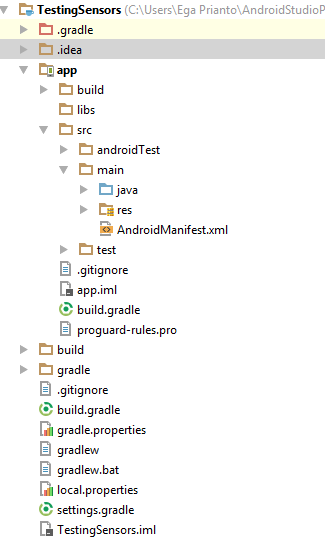
\includegraphics[scale=1]{Gambar/android-studio-structure.png}
	\caption{Tampilan struktur folder pada \textit{project} Android Studio}
	\label{fig:android-studio-structure}
\end{figure}

% 2.1.2 Membuat User Interface
\subsection{Membuat User Interface}
\cite{android_developers}
Pada subbab ini akan dijelaskan bagaimana membuat layout di XML termasuk \textit{text field} dan \textit{button}

% Sub 2.1.2 Hierarki (GUI) untuk Aplikasi Android
\subsubsection{Hierarki \textit{Graphical User Interface} (GUI) untuk Aplikasi Android}
GUI untuk aplikasi Android dibuat dengan hierarki dari objek View dan ViewGroup (Gambar \ref{fig:viewgroup}). Objek-objek dari View biasanya adalah \textit{UI(User Interface) Widgets} seperti \textit{button} atau \textit{text field}. Objek-objek dari ViewGroup tidak terlihat oleh \textit{view containers} yang mendefinisikan bagaimana \textit{child views} ditata seperti \textit{grid} atau \textit{vertical list}.

\begin{figure}[htbp]
	\centering
		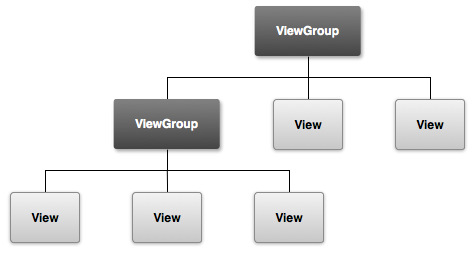
\includegraphics[scale=1]{Gambar/viewgroup.png}
	\caption{Illustrasi bagaimana percabangan objek ViewGroup pada \textit{layout} dan mengandung objek View lainnya.}
	\label{fig:viewgroup}
\end{figure}

Android menggunakan file XML yang berkorespondesi kepada \textit{subclasses} dari View dan ViewGroup, sehingga UI dapat didefinisikan dalam XML menggunakan hierarki dari elemen UI.

\subsubsection{Attribut-attribut Objek View}
Pada subbab ini akan dijelaskan attribut-attribut object View yang digunakan dalam membuat GUI pada file activity\_main.xml
\begin{itemize}
	\item \textbf{android:id}
	Attribut ini merupakan pengidentifikasi dari suatu view. Attribut ini dapat digunakan untuk menjadi referrensi object dari kode aplikasi seperti membaca dan memanipulasi objek tersebut (Akan dijelaskan lebih lanjut pada subbab \ref{sec:activity}). Tanda '@' dibutuhkan ketika mereferensi object dari suatu XML. Tanda '@' tersebut diikuti dengan tipe (id pada kasus ini), \textit{slash}, dan nama (edit\_message pada kode \ref{lst:attribute-view}). Tanda tambah (+) sebelum tipe hanya dibutuhkan jika ingin mendefinisikan \textit{resource ID} untuk pertama kalinya.
	\item \textbf{android:layout\_width} dan \textbf{android:layout\_height}
	Attribut ini digunakan untuk mendefinisikan panjang dan lebar dari suatu objek View. Daripada menggunakan besar spesifik untuk panjang dan lebarnya, lebih baik menggunakan "wrap\_content" yang menspesifikasi viewnya hanya akan sebesar yang dibutuhkan untuk memuat konten-konten dari View. Jika menggunakan "match\_parent" pada kasus kode \ref{lst:attribute-view} View akan memenuhi layar, karena besarnya akan mengikuti besar dari paretnya LinearLayout.


	\item \textbf{android:hint}
	Attribut ini merupakan \textit{default string} untuk di tampilkan ketika objek View kosong. Daripada menggunakan \textit{hard-coded string} sebagai \textit{nilai} untuk ditampilkan, \textit{value} "@string/edit\_message" mereferensi ke sumber string pada file yang berbeda. Karena mereferensi ke sumber konkrit, maka tidak dibutuhkan tanda tambah (+). Nilai string ini akan di simpan pada file Strings.xml yang ditunjukkan pada Kode \ref{lst:string-xml}.
	\begin{lstlisting}[caption={Contoh kode pada string.xml},label={lst:string-xml},language=xml]
	<resources>
    <string name="app_name">MyFirstAndroidApp</string>
    <string name="edit_message">Ini adalah hint</string>
    <string name="button_send">Send</string>
	</resources>

\end{lstlisting}


	\item \textbf{android:onClick}
	Attribut ini akan memberitahu \textit{system} untuk memanggil method yang sesuai namanya (contoh pada kode \ref{lst:attribute-view} adalah \textbf{sendMessage()}) di Activity ketika pengguna melakukan klik pada \textit{button} tersebut. Agar \textit{system} dapat memanggil method yang tepat, method tersebut harus memenuhi kriteria berikut.
	\begin{itemize}
		\item \textit{Access Modifier} haruslah \textit{public}.
		\item Harus \textit{void return value}nya.
		\item Mempunyai View sebagai parameter satu-satunya. View ini akan diisi dengan View yang di klik.
	\end{itemize}
\begin{lstlisting}[caption={Contoh kode file XML pada folder layout},label={lst:attribute-view},language=xml]
	<LinearLayout
		xmlns:android="http://schemas.android.com/apk/res/android"
		xmlns:tools="http://schemas.android.com/tools"
		android:layout_width="match_parent"
		android:layout_height="match_parent"
		android:orientation="horizontal">
		<EditText android:id="@+id/edit_message"
				android:layout_weight="1"
				android:layout_width="0dp"
				android:layout_height="wrap_content"
				android:hint="@string/edit_message" />
		<Button
				android:layout_width="wrap_content"
				android:layout_height="wrap_content"
				android:text="@string/button_send"
				android:onClick="sendMessage" />
	</LinearLayout>
\end{lstlisting}
\end{itemize}


\subsection{Activity}
\label{sec:activity}
\cite{android_developers}
Activity adalah suatu hal yang terfokuskan dengan apa yang bisa pengguna lakukan. Hampir semua \textit{Activity} berinteraksi dengan pengguna, jadi kelas Activity akan membuat suatu halaman baru yang bisa ditambahkan dengan konten-konten View. Selain Activity dapat direpresentasikan kepada pengguna dengan halaman \textit{full-screen}, Activity juga dapat direpresentasikan dengan cara lain: seperti halaman \textit{floating} atau tertanam di Activity lain.

\subsubsection{Activity Lifecycle}

\begin{figure}[htbp]
	\centering
		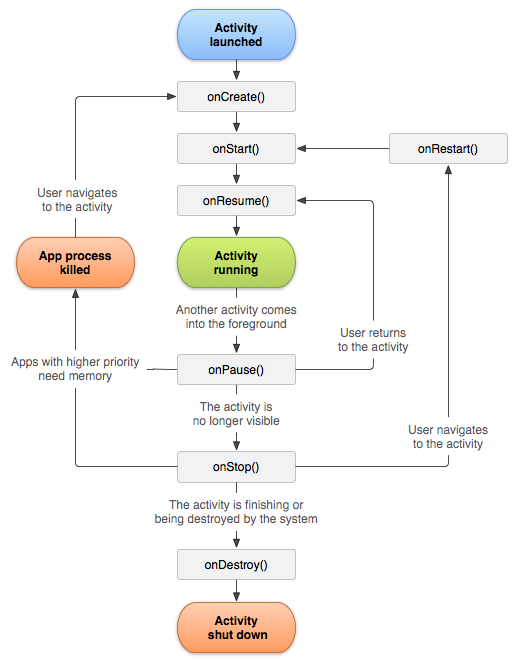
\includegraphics[scale=0.48]{Gambar/activity-lifecycle.png}
	\caption{\textit{State diagram} siklus Activity}
	\label{fig:activity-lifecycle}
\end{figure}

Aktivitas dalam sistem android di atur sebagai \textit{activity stack}. Ketika ada Activity baru yang dimulai, Activity tersebut ditempatkan di paling atas pada \textit{stack} dan menjadi Activity aktif. Activity sebelumnya akan tetap berada di bawah stack, dan tidak akan muncul lagi sampai Activity yang baru berakhir. 

Activity didasari dari empat kondisi:
\begin{itemize}
	\item Jika Activity berada di latar depan pada layar, Activity tersebut sedang aktif.
	\item Jika Activity sudah tidak terfokuskan tetapi masih dapat terlihat, Activity tersebut sedang berhenti sementara. Pada kondisi ini Activity tersebut masih berjalan, tapi bisa diberhentikan ketika system berada dalam situasi kekurangan memori.
	\item Jika suatu Activity benar-benar dihalangi oleh Activity lain, Activity tersebut telah berhenti. Activity tersebut akan tetap mengingat seluruh keadaan dan infomasi anggota tetapi, Activity tersebut tidak lagi terlihat oleh pengguna jadi tampilan jendelanya akan tersembunyi dan seringkali akan diberhentikan Activitynya ketika system membutuhkan memori.
	\item Jika suatu Activity sedang berhenti sementara atau berhenti total, sistem dapat membuang Activity dari memory dengan cara menanyakan kepada pengguna untuk memberhentikannya atau langsung diberhentikan oleh sistem. Jika Activity tersebut ditampilkan lagi kepada pengguna, Activity tersebut harus memulai dari awal dan kembali ke keadaan sebelumnya.
\end{itemize}
Gambar \ref{fig:activity-lifecycle} menunjukkan pentingnya alur keadaan dari suatu Activity. Gambar segi empat merepresentasikan \textit{callback methods} yang dapat diimplementasikan untuk melakukan operasi ketika Activity berubah kondisi. Oval berwarna merupakan kondisi-kondisi utama dari suatu Activity.
Ada 3 \textit{key loops} untuk memantau suatu Activity:
\begin{itemize}
	\item \textit{Entire lifetime} terjadi diantara pemanggilan pertama pada onCreate(Bundle) sampai ke satu pemanggilan akhir onDestroy(). Suatu Activity akan melakukan semua persiapan pada kondisi umum pada method onCreate(), dan melepaskan seluruh sisa pemrosesan pada method onDestroy().
	\item \textit{Visible lifetime} terjadi antara pemanggilan onStart() sampai pemanggilan yang sesuai pada onStop(). Pada tahap ini pengguna dapat melihat Activity pada layar meskipun tidak berada pada \textit{foreground} dan berinteraksi dengan pengguna.
	\item \textit{Foreground lifetime} terjadi antara pemanggilan method onResume() sampai ke satu pemanggilan akhir onDestroy(). Pada tahap ini Activity berada di depan semua Activity lainnya dan sedang berinteraksi dengan user.
\end{itemize}


\subsection{Android Sensor Framework}
\label{sec:android_sensor_framework}
\cite{android_developers}Sebagian besar dari perangkat android sudah memiliki sensor yang mengukur gerakan, orientasi, dan berbagai keadaan lingkungan. Sensor-sensor ini dapat memberikan data mentah dengan tingkat akurasi yang tinggi. Sensor ini juga berguna untuk memantau pergerakan tiga dimensi atau posisi perangkat. Sensor ini juga dapat memantau perubahan keadaan lingkungan yang dekat dengan perangkat. 
Android mendukung tiga kategori sensor:
\begin{itemize}
	\item \textbf{Sensor gerak}
	Sensor-sensor ini mengukur akselerasi dan rotasi pada tiga sumbu. Kategori sensor ini meliputi \textit{accelerometers}, sensor gravitasi, \textit{gyroscope}, dan rotasi vektor. 
	\item \textbf{Sensor keadaan lingkungan}
	Sensor-sensor ini mengukur berbagai keadaan lingkungan seperti suhu udara, tekanan, pencahayaan, dan kelembaban. Kateori sensor ini termasuk barimeter, fotometer dan termometer.
	\item \textbf{Sensor posisi}
	Sensor-sensor ini mengukur posisi perangkat. Kategori sensor ini meliputi sensor orientasi dan magnetometer.
\end{itemize}
Android Sensor Framework membantu developers untuk mengakses berbagai jenis sensor. Beberapa sensor berbasis perangkat keras dan beberapa sensor berbasis perangkat lunak. Sensor berbasis perangkat keras mendapatkan data dengan langsung mengukur sifat lingkungan tertentu, seperti percepatan, kekuatan medan geomagnetik, atau perubahan sudut. Sensor berbasis perangkat lunak mendapatkan data dari satu atau lebih sensor berbasis perangkat keras. Sensor berbasis perangkat lunak ini juga terkadang disebut sensor virtual atau sensor sintetis. Pada tabel berikut akan dirincikan tipe-tipe setiap sensor posisi dan gerak, deskripsi, dan penggunaan umumnya.

\begin{table}[htbp]
	\centering
	\caption{Tipe-tipe Sensor pada Android}
\begin{tabular}{|p{6.3cm}| p{1.5cm}| p{5cm}| p{2.4cm}|} 
\hline
Sensor & Tipe & Deskripsi & Penggunaan umum\\ \hline
TYPE\_ACCELEROMETER & Perangkat Keras & Mengukur percepatan dalam \(m/s^2\) yang terjadi pada perangkat di semua tiga sumbu fisik (x,y,z), termasuk percepatan gravitasi. & Deteksi gerak(goncangan, keseimbangan, dan lain-lain)\\ \hline
TYPE\_GRAVITY & Perangkat Lunak atau Perangkat Keras & Mengukur percepatan gravitasi dalam \(m/s^2\) yang terjadi pada perangkat di tiga sumbu fisik (x,y, dan z) & Deteksi gerak(goncangan, keseimbangan, dan lain-lain)\\ \hline
TYPE\_GYROSCOPE & Perangkat Keras & Mengukur rata-rata rotasi sudut dalam \(rad/s\) di tiga sumbu fisik (x,y, dan z). & Deteksi rotasi (putaran, belokan, dan lain-lain).\\ \hline
TYPE\_LINEAR\_ACCELERATION & Perangkat Lunak atau Perangkat Keras & Mengukur percepatan dalam \(m/s^2\) yang terjadi pada perangkat di semua tiga sumbu fisik (x,y,z), tidak termasuk percepatan gravitasi. & Memantau percepatan pada suatu sumbu.\\ \hline
TYPE\_MAGNETIC\_FIELD & Perangkat Keras & Mengukur medan magnet sekitar untuk semua tiga sumbu fisik (x,y, dan z) di satuan \(\mu T\). & Membuat Kompas.\\ \hline
TYPE\_ORIENTATION & Perangkat Lunak & Mengukur derajat rotasi yang terjadi pada perangkat pada semua tiga sumbu fisik (x,y, dan z). & Menentukan posisi perangkat \\ \hline
TYPE\_ROTATION\_VECTOR & Perangkat Lunak dan Perangkat Keras & Mengukur orisentasi dari suatu perangkat dengan menyediakan tiga element dari vektor rotasi perangkat. & Deteksi gerak dan deteksi rotasi.\\ \hline
\end{tabular}
\end{table}
\subsubsection{Sistem Koordinat Sensor}
\label{sec:sistem_koordinat_sensor}
Pada umumnya, sensor framework menggunakan sistem tiga sumbu koordinat standar untuk mengekspresikan nilai data. Sebagian besar sensor sistem koordinat didefinisikan relatif terhadap layar perangkat bila perangkat dibuat dalam orientasi standar (lihat Gambar \ref{fig:axis-device})
\begin{figure}[htbp]
	\centering
		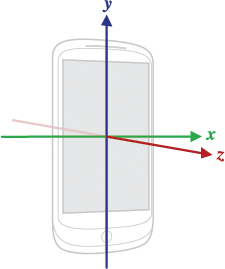
\includegraphics[scale=1]{Gambar/axis-device.png}
	\caption{Sistem koordinat (relatif dengan perangkatnya) yang digunakan oleh Sensor API}
	\label{fig:axis-device}
\end{figure}
Sensor-sensor yang menggunakan sistem tiga sumbu seperti Gambar \ref{fig:axis-device} adalah sebagai berikut :
\begin{itemize}
	\item Accelerometer
	\item Sensor Gravitasi
	\item Gyroscope
	\item Sensor Percepatan Linear
	\item Sensor Medan Geomagnetik
\end{itemize}
Koordinat sistem yang sumbunya tidak tertukar ketika orientasi perangkat berubah. Sistem koordinat sensor tidak pernah berubah seiring perangkatnya bergerak. Dalam aplikasi android tidak dapat diassumsikan bahwa standar orientasi perangkat android adalah \textit{portrait}. Kebanyakan perangkat \textit{Tablet} standar orientasinya adalah \textit{landscape}. Sistem koordinat sensor selalu di dasarkan pada orientasi dasar dari suatu perangkat android.
\subsubsection{Struktur Nilai yang Dikembalikan oleh Sensor}
Nilai dari sensor akan didapatkan ketika ada perubahan nilai pada sensor. Setiap sensor memiliki ketelitian perubahan nilai yang berbeda-beda. Nilai ini akan didapatkan dengan tipe data array of float. Besar dan isi dari array tergantung pada sensor yang sedang di pantau.\\
\textbf{TYPE\_ACCELEROMETER}\\
Semua nilai didefinisikan sebagai satuan \(m/s^2\)
\begin{itemize}
	\item values[0]: Percepatan yang terjadi pada sumbu x dikali -1
	\item values[1]: Percepatan yang terjadi pada sumbu y dikali -1
	\item values[2]: Percepatan yang terjadi pada sumbu z dikali -1
\end{itemize}
Sensor ini mengukur percepatan(\(Ad\)) yang diterapkan pada perangkat. Sensor tersebut dapat mengukur percepatan dengan mengukur gaya(\(Fs\)) yang terjadi pada sensor menggunakan relasi berikut:
\[
	Ad = -\Sigma Fs / mass
\]
Secara khusus, gravitasi selalu mempengaruhi percepatan yang diukur :
\[
	Ad =  -g -\Sigma F / mass
\]
Karena inilah ketika perangkat android sedang diam, accelerometer membaca percepatan gravitasi sebesar \(g = 9.81m/s^2\).
Demikian pula ketika perangkat android sedang dalam keadaan jatuh bebas. Perangkat akan mempercepat menuju ke tanah pada percepatan \(9.81 m/s^2\), sehingga accelerometer membaca percepatan total sebesar \( 0 m/s^2\). 
Suatu saat akan di butuhkan untuk mengukur percepatan asli yang terjadi pada perangkat, sehingga kontribusi gravitasi harus di eliminasi. Hal ini bisa dilakukan dengan menerapkan \textit{high-pass} filter. Sebaliknya, \textit{low-pass} filter dapat digunakan untuk mendapatkan nilai gravitasi saja. 
\begin{lstlisting}[caption={Implementasi \textit{low-pass} filter},label={lst:low-pass-filter},language=java]
	 public void onSensorChanged(SensorEvent event)
     {
          // alpha dikalkulasikan sebagai t / (t + dT)
          // dengan t adalah low-pass filter's time-constant
          // dan dT, rata-rata event tersampaikan

          final float alpha = 0.8;

          gravity[0] = alpha * gravity[0] + (1 - alpha) * event.values[0];
          gravity[1] = alpha * gravity[1] + (1 - alpha) * event.values[1];
          gravity[2] = alpha * gravity[2] + (1 - alpha) * event.values[2];

          linear_acceleration[0] = event.values[0] - gravity[0];
          linear_acceleration[1] = event.values[1] - gravity[1];
          linear_acceleration[2] = event.values[2] - gravity[2];
     }
\end{lstlisting}
\textit{Low-pass} filter dapat diimplementasikan pada kode \ref{lst:low-pass-filter}\\
\textbf{TYPE\_MAGNETIC\_FIELD}\\
Sensor ini mengukur medan magnet sekitar perangkat pada sumbu X,Y, dan Z dalam satuan micro-Tesla.\\
\textbf{TYPE\_GYROSCOPE}\\
Sensor ini mengukur rata-rata perputaran pada perangkat yang berputar di sumbu X,Y, dan Z dalam satuan radians/second. Sistem koordinat yang digunakan sama dengan sistem koordinat pada sensor percepatan(Accelerometer). Jika perangkat berputar berlawanan arah jarum jam pada sumbu tertentu, maka rotasi yang terjadi akan bernilai positif. Perhatikan bahwa standar perputaran ini adalah definisi matematika standar pada rotasi positif.
\begin{itemize}
	\item values[0]: Percepatan angular pada sumbu X.
	\item values[1]: Percepatan angular pada sumbu Y.
	\item values[2]: Percepatan angular pada sumbu Z.
\end{itemize}
Biasanya keluaran dari gyroscope terintegrasi dari waktu ke waktu untuk menghitung rotasi yang menggambarkan perubahan sudut atas langkah waktu, misalnya pada kode \ref{lst:gryoscope-example}
\begin{lstlisting}[caption=contoh implementasi gyroscope,label={lst:gryoscope-example},language=java]
	  private static final float NS2S = 1.0f / 1000000000.0f;
     private final float[] deltaRotationVector = new float[4]();
     private float timestamp;

     public void onSensorChanged(SensorEvent event) {
          // Pada tahapan ini delta rotasi akan dikalikan dengan rotasi saat ini
          // setelah mengomputasinya dari data gyro.
          if (timestamp != 0) {
              final float dT = (event.timestamp - timestamp) * NS2S;
              // Sumbu dari rotasi, masih belum di normalisasi.
              float axisX = event.values[0];
              float axisY = event.values[1];
              float axisZ = event.values[2];

              // Menghitung percepatan angular
              float omegaMagnitude = sqrt(axisX*axisX + axisY*axisY + axisZ*axisZ);

              // Normalisasi rotasi vektor jika cukup besar untuk mendapatkan sumbunya.
              if (omegaMagnitude > EPSILON) {
                  axisX /= omegaMagnitude;
                  axisY /= omegaMagnitude;
                  axisZ /= omegaMagnitude;
              }

              // Integrate around this axis with the angular speed by the time step
              // in order to get a delta rotation from this sample over the time step
              // We will convert this axis-angle representation of the delta rotation
              // into a quaternion before turning it into the rotation matrix.
              float thetaOverTwo = omegaMagnitude * dT / 2.0f;
              float sinThetaOverTwo = sin(thetaOverTwo);
              float cosThetaOverTwo = cos(thetaOverTwo);
              deltaRotationVector[0] = sinThetaOverTwo * axisX;
              deltaRotationVector[1] = sinThetaOverTwo * axisY;
              deltaRotationVector[2] = sinThetaOverTwo * axisZ;
              deltaRotationVector[3] = cosThetaOverTwo;
          }
          timestamp = event.timestamp;
          float[] deltaRotationMatrix = new float[9];
          SensorManager.getRotationMatrixFromVector(deltaRotationMatrix, deltaRotationVector);
          // User code should concatenate the delta rotation we computed with the current rotation
          // in order to get the updated rotation.
          // rotationCurrent = rotationCurrent * deltaRotationMatrix;
     }
     }
\end{lstlisting}
Dalam prakteknya, gyroscope \textit{noise} dan \textit{offset} akan menyebabkan beberapa kesalahan yang harus dikompensasi. Cara untuk mengkompensasinya biasanya dilakukan dengan menggunakan informasi dari sensor lain.\\
\textbf{TYPE\_GRAVITY}\\
Sensor ini menunjukkan arah dan besarnya vektor gaya gravitasi. Sensor ini mengembalikan nilai dengan satuan \(m/s^2\). Sistem koordinat sama seperti sistem koordinat yang umum digunakan sensor percepatan. 

Catatan: Bila perangkat sedang diam, maka keluaran dari sensor gravitasi harus identik dengan accelerometer. \\
\textbf{TYPE\_LINEAR\_ACCELERATION}\\
Sensor yang menunjukkan percepatan pada setiap sumbu perangkat, tidak termasuk percepatan yang terjadi karena gravitasi. Nilai diberikan dalam satuan \(m/s^2\). Sistem koordinat yang digunakan sama seperti sistem koordinat yang digunakan sensor percepatan. Keluaran dari sensor accelerometer, gravitasi dan percepatan linear harus mengikuti aturan berikut:
\[
	percepatan = gravitasi + percepatan linear
\]\\
\textbf{TYPE\_ORIENTATION}\\
Semua nilai adalah sudut dalam derajat.
\begin{itemize}
	\item values[0]: Azimuth, sudut diantara arah magnetik utara dengan sumbu y, sekitar sumbu z (0 sampai 359). 0 = Utara, 90 = Timur, 180 = Selatan, 270 = Barat
	\item values[1]: Pitch, rotasi sekitar sumbu x (-180 sampai 180), dengan nilai positif ketika sumbu x bergerak menuju sumbu y.
	\item values[2]: Roll, perputaran sekitar sumbu y (-90 sampai 90) pada kondisi potrait, sensor akan bernilai 0. Pada kondisi landscape ke kanan sensor akan bernilai 90 dan sebaliknya yaitu kondisi landscape ke kiri sensor akan bernilai -90.
\end{itemize}

Catatan: Definisi ini berbeda dengan definisi yaw, pitch, dan roll yang digunakan pada aviasi yang sumbu X adalah sepanjang sisi bidang.

Catatan: Sensor ini sudah tidak digunakan lagi(deprecated), yang digunakan sekarang adalah sensor rotasi vector.\\
\textbf{TYPE\_ROTATION\_VECTOR}\\
Sensor ini merepresentasikan orientasi perangkat dengan kombinasi dari sumbu dan sudut. Perangkat akan di putar sebesar sudut \(\theta\) mengelilingi sumbu \(x,y,z\). Tiga elemen dari vektor rotasi adalah (\(x \sin (\frac{\theta}{2}), y \sin (\frac{\theta}{2}), z \sin (\frac{\theta}{2})\)), sehingga besarnya vektor rotasi sama dengan \(\sin (\frac{\theta}{2})\), dan arah vektor rotasi sama dengan sumbu rotasi. Tiga elemen dari vektor rotasi sama dengan tiga komponen terakhir pada unit quaternion(\(\cos (\frac{\theta}{2}),x \sin (\frac{\theta}{2}), y \sin (\frac{\theta}{2}), z \sin (\frac{\theta}{2})\)) yang dijelaskan pada subbab \ref{sec:teori_quaternion}. Elemen dari vektor rotasi tak memiliki satuan. Sistem koordinat yang digunakan sama dengan sistem koordinat yang digunakan pada sensor percepatan. Referensi koordinat didefinisikan sebagai basis orthonormal, yaitu:
\begin{itemize}
	\item X didefinisikan sebagai perkalian dot product \textbf{Y.Z}
	\item Y merupakan tangensial ke tanan pada lokasi perangkat saat ini dan menunjuk ke arah utara. 
	\item Z menghadap ke langit dan tegak lurus dengan tanah. Untuk lebih jelasnya dapat dilihat pada Gambar \ref{fig:axis-globe}
	\begin{figure}[htbp]
	\centering
	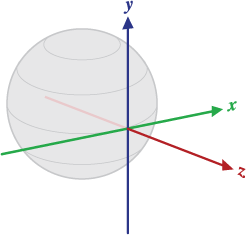
\includegraphics[scale=1]{Gambar/axis-globe.png}
	\caption{Sistem koordinat sensor rotasi vektor terhadap Bumi} 
	\label{fig:axis-globe}
	\end{figure}
	\item values[0]: \(x \sin (\frac{\theta}{2})\)
	\item values[1]: \(y \sin (\frac{\theta}{2})\)
	\item values[2]: \(z \sin (\frac{\theta}{2})\)
	\item values[3]: \(\cos (\frac{\theta}{2})\)
	\item values[4]: Perkiraan akurasi (dalam radians) (-1 jika tidak tersedia) 
\end{itemize}
\section{Google VR SDK}
\label{sec:google_vr_sdk}
Google VR SDK\cite{google_vr_developers} digunakan untuk membantu dalam pembuatan aplikasi Virtual Reality pada \textit{smartphone}. Google VR SDK memberikan beberapa fitur sebagai berikut :
\begin{itemize}
	\item \textbf{Binocular rendering}: Fitur untuk tampilan layar terpisah untuk masing-masing dalam pandangan VR.
	\item \textbf{Spatial audio}: Fitur untuk mengeluarkan suara yang datang dari daerah-daerah tertentu dari dunia VR.
	\item \textbf{Head movement tracking}: Fitur untuk mendapatkan memperbaharui pengelihatan dunia VR yang sesuai dengan gerakan kepala pengguna.
	\item \textbf{Trigger input}: Fitur untuk memberikan input pada dunia VR dengan menekan tombol.
\end{itemize}

Ada beberapa persyaratan untuk menggunakan Google VR SDK, persyaratan tersebut adalah:
\begin{itemize}
	\item Android Studio versi 1.0 atau lebih.
	\item Android SDK versi 23
	\item Gradle versi 23.0.1 atau lebih. Android Studio akan membantu meningkatkan versinya jika versinya terlalu rendah.
	\item Perangkat Android fisik yang menjalankan Android versi 4.4 (KitKat) atau lebih.
\end{itemize}

Dalam membuat aplikasi Google Cardboard VR membutuhkan beberapa API(Application Program Interface) dari Google VR SDK. API-API umum yang akan digunakan adalah sebagai berikut. 
\begin{itemize}
	\item API audio: API untuk mengimplementasikan \textbf{\textit{Spatial Audio}} (Metode untuk menspasialisasikan sumber suara dalam ruang tiga dimensi).
	\item API base: API untuk fondasi dari suatu aplikasi Google VR.
\end{itemize}

\subsection{API Audio}
\label{sec:api_audio}
\cite{google_vr_developers}
API ini membantu developer untuk menspasialisasikan sumber suara dalam tiga dimensi, termasuk jarak dengan tinggi isyarat sumber suara. Pada API ini hanya terdapat satu class utama yaitu \textbf{GvrAudioEngine}. \textbf{GvrAudioEngine} mampu memutarkan suara secara spasial dalam dua cara yang berbeda :
\begin{itemize}
	\item Metode pertama dikenal sebagai \textit{Sound Object rendering}. Metode ini memungkinkan pengguna membuat sumber suara virtual dalam ruang tiga dimensi.
	\item Metode kedua memungkinkan pengguna untuk memutar kembali rekaman \textit{Ambisonic soundfield}. Rekaman \textit{Ambisonic soundfield} adalah file audio \textit{multi-channel} yang telah terspasialisasi.
\end{itemize}
API ini juga dapat memutarkan suara secara \textit{stereo}. Kelas \textbf{GvrAudioEngine} memiliki tiga buah \textit{nested class} yaitu:
\begin{itemize}
	\item GvrAudioEngine.DistanceRolloffModel: Kelas ini mendefinisikan konstanta-konstanta yang merepresentasikan perbedaan jarak dari efek model-model rolloff. 
	\item GvrAudioEngine.MaterialName: Kelas ini mendefinisikan konstanta-konstanta yang merepresentasikan bahan permukaan ruangan untuk disesuaikan dengan efek suara pada suatu ruangan.
	\item GvrAudioEngine.RenderingMode: Kelas ini mendefinisikan konstanta-konstanta untuk menyesuaikan dengan mode rendering. Semakin baik kualitas renderin akan semakin besar penggunaan CPU(Central Processing Unit).
\end{itemize}

\subsection{API Base}
\label{sec:api_base}
\cite{google_vr_developers}
API ini digunakan sebagai fondasi dari suatu aplikasi Google VR. Fitur-fitur Binocular rendering, Head movement tracking, dan Trigger input diimplementasikan pada API ini. Kelas-kelas penting yang ada di API ini adalah AndroidCompat, Eye, GvrActivity, GvrView, HeadTransform, Viewport.
\begin{itemize}
	\item AndroidCompat\\
Kelas ini merupakan kelas utilitas untuk menggunakan fitur VR. Fitur-fitur ini mungkin tidak tersedia pada semua versi android. Kelas ini memiliki method-method sebagai berikut:
\begin{itemize}
	\item setSustainedPerformanceMode(Activity activity, boolean enabled): \\
	Method ini digunakan untuk mengubah window android ke mode performa secara berkelanjutan.
	\item public static void setVrModeEnabled (Activity activity, boolean enabled): \\
	Mengatur pengaturan yang tepat untuk "mode VR" pada suatu Activity. Method ini tidak digunakan karena hanya dapat digunakan pada Android N+.
	\item public static boolean trySetVrModeEnabled (Activity activity, boolean enabled): 
	Method ini kegunaanya sama dengan method \textbf{setVrModeEnabled (Activity activity, boolean enabled)}, namun mengembalikan boolean true jika berhasil dan sebaliknya.
\end{itemize}
	\item Eye\\
Kelas ini mendefinisikan detil perenderan stereoskopik mata. Method penting yang dimiliki kelas ini adalah \textbf{public float[] getEyeView ()}. Method ini mengembalikan matriks yang mentransformasikan camera virtual ke mata. Transformasi yang diberikan termasuk melacak rotasi kepala, perubahan posisi dan perubahan IPD(interpupillary distance).
	\item GvrActivity\\
Kelas ini merupakan Activity dasar yang menyediakan integrasi yang mudah dengan headset Google VR. Kelas ini mengekspos kejadian untuk berinteraksi dengan headset Google VR dan menangani detil-detil yang biasa diperlukan saat membuat suatu Activity untuk perenderan VR. Activity ini membuat layar tetap menyala selama perangkat android bergerak. Jika tidak ada pergerakan dari perangkat android maka layar reguler (\textit{wakeclock}) akan ditampilkan. Pada kelas ini terdapat method \textbf{onCardboardTrigger ()} untuk mendeteksi ketika Cardboard Trigger sedang ditarik dan dilepaskan (Magnet yang berada pada sisi Google Cardboard).
	\item GvrView\\
	Kelas ini merupakan kelas View yang menyediakan perenderan VR. Kelas ini didesain untuk berkerja pada mode layar penuh dengan orientasi \textit{landscape} atau \textit{reverse landscape}. Kelas View ini dapat digunakan dengan mengimplements salah satu Interface perenderan. Interface-interface tersebut adalah:
	\begin{itemize}
		\item GvrView.StereoRenderer: Interface untuk perenderan detil stereoskopik secara abstrak oleh perender.
		\item GvrView.Renderer: Interface untuk mesin yang kompleks yang membutuhkan untuk menangai semua detil perenderan.
	\end{itemize}
Kelas GvrView.Renderer jarang digunakan dan sebaiknya tidak digunakan jika tidak sangat dibutuhkan.
Ketika suatu kelas mengimplement Kelas GvrView.StereoRenderer, kelas tersebut harus mengimplementasikan method-method berikut ini:
\begin{itemize}
	\item \textbf{public void onNewFrame(HeadTransform headTransform)}\\
	method ini terpanggil ketika Framebaru akan digambar. Method ini memungkinkan untuk membedakan antara perenderan pandangan mata dan frame-frame yang berbeda. Setiap operasi per-frame harus tidak spesifik pada satu tampilan saja.
	\item \textbf{public abstract void onDrawEye (Eye eye)}\\
	Method ini meminta untuk menggambar suatu konten dari sudut pandang mata.
	\item \textbf{public abstract void onFinishFrame (Viewport viewport)}\\
	Method ini dipanggil ketika suatu frame telah selesai. Dengan pemanggilan ini, konten frame telah di gambar dan jika koreksi distorsi diaktifkan, koreksi distrosi akan diterapkan. Setiap perendereran pada tahap ini relatif terhadap seluruh permukana, tidak terhadap satu pandangan mata tunggal. 
	\item \textbf{public abstract void onRendererShutdown ()}\\
	Method ini dipanggil ketika thread perender sedang menutup. Melepaskan sumber GL(Graphics Library) dan sedang melakukan penutupan operasi pada thread perender. Dipanggil hanya jika sebelumnya ada pemanggilan method onSurfaceCreated.
	\item \textbf{public abstract void onSurfaceChanged (int width, int height)}\\
	Dipanggil ketika ada perubahan dimensi permukaan. Semua nilai adalah relatif ke ukuran yang dibutuhkan untuk merender sebuah mata.
	\item \textbf{public abstract void onSurfaceCreated (EGLConfig config)}\\
	Method ini dipanggil ketika suatu permukaan dibangun atau dibangun ulang.
\end{itemize}
\item HeadTransform\\
	Method ini mendeskripsikan transformasi kepala secara independen dari setiap parameter mata. Kelas ini digunakan di kelas GvrView.StereoRenderer sebagai parameter pada method \textbf{onNewFrame}. Method-method yang perlu diperhatikan pada kelas ini adalah:
	\begin{itemize}
		\item \textbf{public void getHeadView (float[] headView, int offset)}\\
		Method ini digunakan untuk mendapatkan matriks transformasi dari camera virtual ke kepala. Kepala disini didefinisikan sebagai titik tengah diantara kedua mata. Matriks yang didapatkan akan disimpan pada parameter \textbf{headView}.
		\item \textbf{public void getQuaternion (float[] quaternion, int offset)}\\
		Method ini digunakan untuk mendapatkan quaternion yang merepresentasikan rotasi kepala.
	\end{itemize}
	\item Viewport\\
	Kelas ini didefinisikan sebagai \textit{viewport}(area pandang) berbentuk persegi.
\end{itemize}
\section{Head Motion Detection Menggunakan Camera Inframerah}
\label{sec:head_motion_detection}
\cite{kapoor2001real}Mengangguk kepala dan menggeleng kepala merupakan gerakan non-verbal yang sering digunakan untuk berkomunikasi.  Arah dari pergerakan kepala dapat diperoleh dari posisi pupil pada camera. Posisi pupil pada camera ini digunakan pada observasi diskrit Hidden Markov Model(HMM) berdasarkan pola alat analisa untuk mendeteksi kepala ketika sedang mengangguk atau menggeleng. Sistem ini akan dilatih dan diuji pada data rekaman dari sepuluh pengguna dengan variasi pencahayaan dan ekspresi muka. Sistem ini memiliki tingkat akurasi sebesar 78.46\% berdasarkan pada data tes.
\subsection{Probabilitas Kemungkinan dan Kebebasan}
Terkadang kita memiliki pengetahuan tentang hasil dari suatu eksperimen dan secara alamiah mungkin mempengaruhi hasil pencobaan lainnya. Pengetahuan ini dapat di peroled dengan konsep probabilitas bersyarat. Kemungkinan dari suatu kejadian sebelum mempertimbahkan pengetahuan tambahan disebut juga \textit{prior probability} dari suatu kejadian. Kemungkinan dari hasil penggunaan pengetahuan tambahan disebut dengan \textit{posterior probability} dari suatu kejadian. Probabilitas bersyarat dari suatu kejadian A yang terjadi setelah kejadian B terjadi(\(P(A|B)\)) dengan Peluang B lebih besar dari 0 (\(P(B)>0\)) adalah:
\begin{align*}
	P(A|B) =& \frac{P(A\cap B)}{P(B)}\\
	&atau,\\
	P(A|B) =& \frac{P(A,B)}{P(B)}
\end{align*}
bahkan jika P(B) = 0, masih dapat diselesaikan dengan aturan perkalian:
\[
	P(A\cap B) = P(B)P(A|B) = P(A)P(B|A)
\]
Generalisasi dari aturan ini untuk banyak kejadian adalah sebagai berikut, atau disebut juga sebagai \textit{chain rule}:
\[
	P(A_1\cap ...\cap A_n)=P(A_1)P(A_2|A_1)P(A_3|A_1\cap A_2)...P(A_n|\cap^{n-1}_{i=1} A_i)
\]
\textit{Chain rule} ini akan digunakan dalam Markov Model.
Kejadian A dengan B bersifat independen. Hal ini menyebabkan jika \(P(A\cap B) = P(A)P(B)\) kecuali \(P(B) = 0 \) akan menghasilkan persamaan \(P(A) = P(A|B)\)
\subsection{Markov Model} 
\label{sec:markov-model}
\cite{manning1999natural} 
\begin{figure}[htbp]
	\centering
		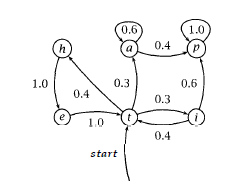
\includegraphics{Gambar/markov-model-example.png}
	\caption{Contoh Markov Model}
	\label{fig:markov-model-example}
\end{figure}
Markov model dapat digunakan ketika ingin memodelkan probabilitas dari suatu urutan linear pada suatu peristiwa. Contohnya, markov model yang digunakan dalam pemodelan urutan tutur perkataan dalam suatu dialog. Selain itu markov model juga digunakan untuk pengenal suara dan lain-lain. 
Deret Markov menggunakan 
Deret Markov dapat merepresentasikan oleh Markov model dengan suatu State Diagram seperti pada gambar \ref{fig:markov-model-example}. Transisi yang mungkin terjadi digambarkan dengan panah yang menghubungkan antar kondisi, dan pada lengkungan panahnya di berikan label probabilitas dari transisi tersebut. Jumlah dari seluruh probabilitas yang keluar dari suatu kondisi akan berjumlah 1. Dalam Markov Model, dapat diketahui bahwa kondisi-kondisi yang akan suatu mesin tempuh, sehingga urutan kondisi atau beberapa fungsi deterministik dapat dijadikan sebagai pengeluaran. 
Probabilitas dari suatu urutan kondisi (yaitu urutan dari variabel-variabel random) \(X_i,...,X_T\) dapat dengan mudah di kalkukasi dengan deret Markov. Deret Markov dapat direpresentasikan dengan persamaan berikut:
\begin{align*}
P(X_1,...,X_T) =& P(X_1)P(X_2|X_1)P(X_3|X_1,X_2)...P(X_T|X_1,...,X_{T-1})\\
=& P(X_1)P(X_2|X_1)P(X_3|X_2)...P(X_T|X_1,...,X_{T-1})\\
=& \pi_{X_1} \Pi^{T-1}_{t=1} A X_t X_{t+1}
\end{align*}\\
Jadi, dengan Markov Model pada gambar \ref{fig:markov-model-example}, didapatkan:
\begin{align*}
	P(t,i,p) =& P(X_1 = t)P(X_2 = i|X_1 = t)P(X_3 = p|X_2 = i)\\
	 =& 1.0 \times* 0.3 \times* 0.6\\
	 =& 0.18
\end{align*}

\subsubsection{Hidden Markov Models}
\label{sec:hidden-markov-models}
\cite{manning1999natural} 
Pada HMM(Hidden Markov Models), tidak dapat diketahui urutan kondisi yand dilewati model, tetapi hanya beberapa fungsi probabilistik saja yang diketahui. HMM berguna ketika dapat memikirkan peristiwa secara probabilistik yang menghasilkan peristiwa muka. 

\textbf{Bentuk Umum HMM}\\
\cite{manning1999natural} 
HMM dispesifikasikan dengan (\(S,K,II,A,B)\), dimana S dengan K adalah kumpulan kondisi dan keluaran alphabet, dan II, A, dan B adalah probabilitas untuk kondisi awal, kondisi transisi, dan emisi simbul, secara berturut-turut. Notasi-notasi tersebut akan dijelaskan lebih lanjut pada tabel \ref{tab:hmm-notation}

\cite{manning1999natural} 
\begin{table}%
	\centering
\begin{tabular}{l l}
Kumpulan kondisi  & \(S=\{ s_1,...,s_N\}\)\\
Keluaran alphabet	& \(\{k_1,...,k_M\} = \{1,...,M\}\)\\
\\
Probabilitas kondisi awal & \(II = \{\pi_i\}, i\in S\)\\
Probabilitas kondisi transisi & \(\{a_{ij}\},i,j\in S\)\\
Probabilitas emisi simbol & \(\{a_{ij}\},i,j\in S\)\\
\\
Deretan kondisi	& \(x= (X_,...,X_{T+1}) X_t : s \stackrel{}{\rightarrow} \{1,...,M\}\)\\
Deretan keluaran & \(O= (o_1,...,o_T) O_t \in K\)
\end{tabular}
\caption{Notasi yang digunakan dalam HMM}
\label{tab:hmm-notation}
\end{table}


\textbf{Mencari Probabilitas dari Suatu Observasi}
\cite{manning1999natural} 
Diberikan suatu urutan observasi \(O = (o_1,...,o_T)\) dan suatu model \(\mu = (A,B,II)\), yang ingin dicari adalah bagaimana mengkalukasi \(P(O|\mu )\) secara efisien. Proses ini sering disebut juga sebagai \textit{decoding}. Untuk semua deret kondisi \(X = (X_1,...,X_{T+1})\),
\begin{align*}
	P(O|X,\mu ) =& \Pi^{T}_{t=1} P(o_t|X_t,X_t+1,\mu )\\
		=& b_{X_1 X_2 o_1}b_{X_2 X_3 o_2}... b_{X_T X_{T+1}o_T}
\end{align*}
dan, 
\[
	P(X|\mu ) = \Pi_{X_1}a_{X_1 X_2}a_{X_2 X_3}...a_{X_T X_{T+1}}\\
\]
adapun,
\[
	P(O,X|\mu ) = P(O|X,\mu ) P(X|\mu )
\]
olehkarena itu, 
\begin{align*}
	P(O|\mu ) =& \Sigma_X P(O|X,\mu ) P(X|\mu )\\
	=& \Sigma_{X_1 ...X_{T+1}} \pi X_1 \Pi^{T}_{t=1} a_{X_t X_{T+1}}b_{X_t X_{t+1}o_T}
\end{align*}
\cite{manning1999natural} 
Penurunan ini cukup terang-terangan. Sayangnya, evaluasi langsung dari ekspresi yang dihasilkan tersebut sangatlah tidak efisien. Untuk kasus umum (kasus yang dapat dimulai pada kondisi apapun, dan pindah ke kondisi lain pada setiap tahapnya), kalkukasinya membutuhkan \((2T+1).T^{T+1}\) Untuk menangai kompleksitas ini dapat menggunakan teknik umum yaitu \textit{dynamic programming memoization} yang mengingat sebagian hasil dibandingkan harus menghitung ulang kembali. Untuk algoritma seperti HMM, \textit{dynamic programming} secara umum dideskripsikan dalam bentuk dari \textit{trellises}(bisa juga disebut dengan \textit{laticces}). \textit{Trellis} dapa merekan probabilitas semua \textit{subpaths} awal dari suatu HMM yang berakhir pada kondisi tertentu pada waktu tertentu. Probabilitas dari \textit{subpaths} yang lebih panjang dapat digunakan untuk suatu hal dari \textit{subpaths} yang lebih pendek.
\section{Teori Quaternion}
\label{sec:teori_quaternion}

Pada Android SDK \textbf{SensorEvent.values} \cite{android_developers} tipe sensor \textbf{Sensor.TYPE\_ROTATION\_VECTOR}, yaitu tipe sensor yang mendeteksi vektor perputaran pada \textit{smartphone}. Tipe sensor ini dijelaskan akan mengembalikan nilai-nilai dari komponen quaternion. 
Quaternion\cite{kuipers:1999} adalah objek penggabungan dari suatu skalar dengan suatu vektor, sesuatu yang tidak dapat didefinisikan dalam aljabar linear biasa. 

\subsection{Struktur Ajabar}
Struktur-Struktur aljabar yang digunakan adalah Bilangan Kompleks, Konjugasi Kompleks, \textit{Quaternion Algebra}, dan Operasi-operasi pada \textit{Quaternion}.

\subsubsection{Bilangan Kompleks}

Dalam matematika, bilangan kompleks adalah bilangan yang berbentuk\\
\[
	a+bi
\]\cite{kuipers:1999}\\
dan \(a\) dengan \(b\) merupakan bilangan riil, dan \(i\) merupakan bilangan imajiner tertentu yang memiliki sifat \(i^2=-1\).

Berikut notasi-notasi bilangan kompleks :
\begin{itemize}
	\item Penjumlahan\\
	\[
	 (a + bi) + (c + di) = (a+c) + i(b+d)
	\]\\
	\item Perkalian\\
	\[
	 (a + bi)(c + di) = (ac−bd) + (bc+ad)i
	\]
	\item Pengurangan\\
	\[
	 (a + bi) - (c + di) = (a-c) + i(b-d)
	\]
	\item Pembagian\\
	\[
	 \frac{(a + bi)}{(c + di)} = \frac{(ac+bd)}{c^2+d^2} + i \frac{bc-ad}{c^2+d^2}
	\]
\end{itemize}
Terlihat jelas bahwa penjumlahan dan perkalian untuk bilangan kompleks keduanya adalah assosiatif dan komutatif. Detilnya dapat dilihat dengan persamaan di bawah ini.
\[
	(a+ib) + (c+id) = (a+c) + i(b+d)\\
	(c+id) + (a+ib) = (c+a) + i(d+b)
\]
Karena penjumlahan untuk bilangan riil bersifat komutatif:
\[
	a+c = c+a\\
	b+d = d+b
\]

Bilangan kompleks dapat digunakan untuk rotasi dua dimensi. Dengan \(a = \cos (\frac{\theta}{2})\), dan \(b = \sin(\frac{\theta}{2})\), kemudian akan dikalikan dengan vektor yang ingin di putar, dengan sumbu putar adalah titik pusat.


\subsubsection{Konjugasi Kompleks}
\cite{kuipers:1999}Berhubungan dengan bentuk umum bilangan kompleks,
\[
	z = a + ib
\]\\
satu bilangan dikatakan konjugasi kompleks jika
\[
	\bar{z} = a - ib
\]\\
Dari kedua persamaan diatas dapat dihasilkan :
\[
	z + \bar{z} = 2a
\]dan,
\[
	z \bar(z) = a^2 +b^2 = |z|^2
\]

\subsection{\textit{Quaternion Algebra} dan Operasi-operasi pada Quaternion}
\cite{kuipers:1999}Pada buku "Quaternions and Rotation Sequences : A Primer with Applications to Orbits, Aerospace, and Virtual Reality" disebutkan bahwa tingkat empat bilangan sangat kompleks, dinamakan quaternion. Dari penemuan ini dibuat aturan:
\[
	i^2 = j^2 = k^2 = ijk = -1
\]
untuk beoperasi dengan vektor bagian dari suatu quaternion.
Untuk hasil dari perkalian dua \textit{quaternion} memiliki aturan yang lebih rumit, sehingga memiliki aturan-aturan khusus. Berikut aturan-aturan khususnya :
\begin{equation}
	\begin{split}
	& ij = k = -ji\\
	& jk = i = -kj\\
	& ki = j = -ik	
	\end{split}
\label{eq:persamaan_khusus_aturan_quaternion}
\end{equation}\\
Perhatikan bahwa ketiga persamaan diatas mirip dengan cross product vektor sesuai dengan aturan tangan kanan (\textit{right-hand rule}). Dapat di katakan pada Gambar \ref{fig:right-hand-rule}, \(A\) berperan sebagai \(i\), \(B\) berperan sebagai \(j\), dan \(C\) berperan sebagai \(k\). Sehingga terpenuhi sesuai dengan persaman-persamaan \ref{eq:persamaan_khusus_aturan_quaternion}\\
\begin{figure}[htbp]
\centering
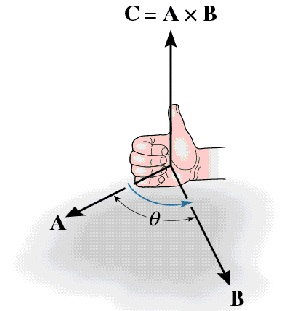
\includegraphics[scale=1]{Gambar/right-hand-rule}
\caption{Right-hand rule dalam \textit{cross product} vektor} 
\label{fig:right-hand-rule}
\end{figure}\\
\textit{Quaternion} memiliki persamaan umum yang memiliki empat bilangan riil atau skalar. Persamaan tersebut adalah 
\[
	q = q_0 + i q_1 + j q_2 + k q_3
\]\cite{kuipers:1999}
Sama seperti pada bilangan kompleks, \textit{quaternion} juga memiliki konjugasi kompleksnya. Berikut adalah konjugasi kompleks \textit{quaternion}
\[
	q = q_0 - i q_1 - j q_2 - k q_3
\]
\subsubsection{Operasi pada Quaternion}
Dua buah quaternion dapat dikatakan sama jika dan hanya jika kedua quaternion memiliki komponen yang sama.
\[
	p = p_0 + +ip_1+jp_2+kp_3
\]
dan,
\[
	q = q_0 + i q_1 + j q_2 + k q_3
\]
maka p = q jika dan hanya jika
\[
	p_0=q_0\\
	p_1=q_1\\
	p_2=q_2\\
	p_3=q_3\\
\]
Penjumlahan dari kedua quaternion diatas dapat didefinisikan sebagai komponen penjumlahan yaitu:
\[
	(p+q)=(p_0+q_0)+i(p_1+q_1)+j(p_2+q_2)+k(p_3+q_3)
\]
Perkalian dari kedua quaternion diatas dapat didefinisikan sebagai komponen perkalian yaitu:
\[
	pq = (p_0 + +ip_1+jp_2+kp_3)(q_0 + i q_1 + j q_2 + k q_3)
\]
Begitu pula juga dengan pembagian dan pengurangan.}{}
\ifdefstring{\vbabc}{1}{\chapter{Analisis}
\label{chap:analisis}

\section{Mesin Navigasi KIRI}
\label{sec:mesin_navigasi_kiri}

\subsection{Mekanisme Penarikan}

Untuk mendukung integrasi data antara angkot.web.id dan KIRI, diperlukan adanya penarikan secara berkala terhadap angkot.web.id oleh KIRI. Ada dua alternatif metode yang dipertimbangkan sebagai mekanisme penarikan data ini:

\begin{description}
	\item[Metode \textit{realtime}] Metode ini mendeteksi setiap perubahan yang terjadi pada data angkot.web.id, dan langsung memberi notifikasi kepada KIRI untuk mengambil ulang data yang berubah dari angkot.web.id
	\item[Metode \textit{polling}] Pada metode ini, KIRI akan mengambil data secara berkala dari angkot.web.id, sehingga akan terdapat jeda antara perubahan data dan terbaharuinya data KIRI.
\end{description}

Dari kedua metode tersebut, peneliti memilih untuk menggunakan metode \textit{polling} dengan alasan-alasan sebagai berikut:

\begin{description}
	\item[Lebih sedikit perubahan] Angkot.web.id menggunakan protokol HTTP yang bersifat \textit{conectionless}, sehingga secara alami akan menunggu perintah dari \textit{client}, alih-alih secara aktif memberi notifikasi kepada \textit{client}. Jika menggunakan metode \textit{polling}, KIRI dapat memanfaatkan protokol \textit{Transportation Detail} yang sudah dimiliki oleh angkot.web.id.
	\item[Mengurangi kebutuhan prosesor] Rute pada KIRI dimodelkan dalam bentuk graf, dan sebelum dapat digunakan untuk pencarian graf ini harus dikonstruksi terlebih dahulu. Akibat besarnya data yang digunakan, konstruksi ini akan memakan waktu (kurang lebih 30 detik). Dengan menggunakan metode \textit{realtime}, setiap perubahan data pada kiri.web.id akan mengakibatkan graf ini harus direkonstruksi ulang. Dengan menggunakan metode \textit{polling}, penarikan data dan rekonstruksi graf dapat diatur sedemikian sehingga dilakukan pada saat pengguna sedang tidak aktif.
	\item[Urgensi Perbaikan Data] Peneliti berpendapat bahwa urgensi perbaikan data tidak terlalu tinggi untuk KIRI (bandingkan dengan perubahan harga saham, \textit{realtime GPS monitoring}, dll).
\end{description}

Penulis menetapkan penggunaan metode \textit{polling} selama 24 jam sekali, dan dipilih waktu 0.30 (setengah jam setelah tengah malam) untuk melakukan \textit{polling}. Penetapan waktu ini mempertimbangkan sedikitnya penggunaan KIRI pada saat tengah malam. Jeda setengah jam dilakukan untuk memberikan toleransi terhadap perbedaan waktu komputer beberapa detik, yang mungkin memberikan masalah pada tanggal sistem. 

\subsection{Penyimpanan Data}

Penyimpanan data diusahakan untuk meminimalisir perubahan serta menjaga kompatibilitas dengan versi sebelumnya. Seperti yang telah dibahas pada bab 2, mesin navigasi KIRI menggunakan berkas \verb/tracks.conf/ sebagai jembatan dari basis data menuju mesin navigasi. Berkas inilah yang akan dikonstruksi menjadi graf oleh kelas \verb/Worker/. Peneliti memutuskan untuk tidak mengubah format dari berkas ini, melainkan melakukan modifikasi pada basis data.

Pada basis data, tetap diusahakan untuk meminimalisir perubahan. Dari struktur tabel \verb/tracks/ yang digunakan, diidentifikasi bahwa kolom `internalInfo` tidak digunakan dalam perhitungan (tidak berpengaruh pada konstruksi graf). Oleh sebab itu, kolom ini menjadi kandidat untuk disisipkan informasi terkait dengan penarikan data dari angkot.web.id. Adapun informasi yang harus disimpan adalah:

\begin{itemize}
	\item Penanda bahwa rute ini ditarik dari angkot.web.id
	\item Kode yang mengacu pada basis data angkot.web.id, dalam hal ini \verb/id/.
\end{itemize}

%Peneliti memutuskan untuk menyimpan kedua informasi tersebut dalam kolom \verb/internalInfo/, dengan format "angkotwebid:\textit{id}". Dengan cara ini, trayek yang memiliki \verb/internalInfo/ diawali dengan "angkotwebid:" akan diproses lebih lanjut dengan menarik data dari angkot.web.id. Penarikan data dilakukan dengan mendapatkan \textit{id} yang berada setelah simbol ":", dan menariknya di angkot.web.id dengan perintah \textit{Transportation Detail}. Sebagai contoh, jika ditemukan data dengan \verb/internalInfo/ bernilai "angkotwebid:1", akan ditarik data rute dari alamat \url{https://angkot.web.id/route/transportation/1.json}. Rute yang didapat tersebut kemudian akan dimasukkan ke dalam basis data pada kolom \verb/geodata/.

\subsection{Analisis Aplikasi}

Pada penelitian ini, mesin navigasi KIRI dimodifikasi dengan menambahkan dua kelas baru, yaitu kelas \verb/DataPuller/ yang difungsikan sebagai penarik data dari angkot.web.id, serta kelas \verb/DataPullerException/ untuk mencatat kesalahan pada saat menarik data dari angkot.web.id. Kelas-kelas yang baru serta yang lama digambarkan pada diagram kelas di gambar \ref{fig:3_diagram_kelas_sistem_usulan}.

\begin{figure}
	\centering
	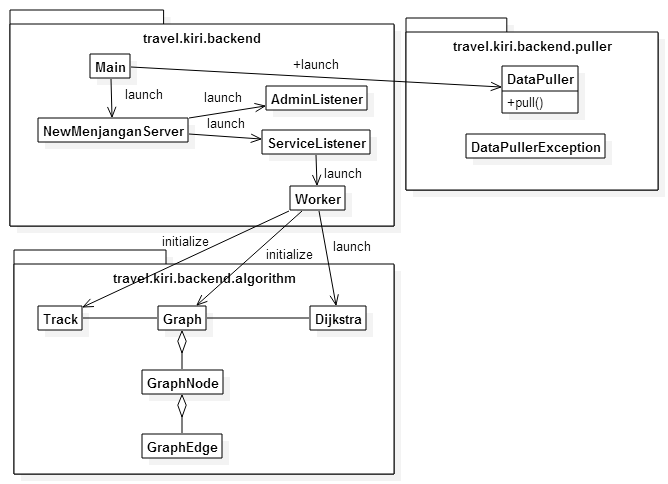
\includegraphics[scale=0.5]{Gambar/3_diagram_kelas_sistem_usulan}
	\caption{Diagram Kelas Sistem Usulan (Tahap Analisis)} 
	\label{fig:3_diagram_kelas_sistem_usulan}
\end{figure}

\section{Angkot.web.id}

Pada dasarnya angkot.web.id tidak diperlukan adanya perubahan, karena KIRI dapat memanfaatkan protokol \textit{transportartion detail}. Namun, untuk keperluan optimasi, ada sedikit perubahan yang dijelaskan pada subbab berikutnya.

\section{Optimasi}

Dengan mekanisme yang sudah dijelaskan di subbab sebelumnya, data pada KIRI dapat tersinkronisasi dengan angkot.web.id. Namun, mekanisme tersebut dirasa tidak optimal. Setiap pukul 0.30, KIRI akan menarik ke-33 rute angkot yang dicatat pada angkot.web.id, terlepas dari apakah ada perubahan pada rute angkot atau tidak. Walaupun hanya menarik 33 rute dan dilakukan pada jam tidak sibuk, peneliti merasa optimasi tetap dibutuhkan sehingga solusi ini skalabel.

Mekanisme \textit{Transportation List} maupun \textit{Transportation Detail} pada angkot.web.id memberikan informasi \textit{updated} yang menunjukkan waktu terakhir rute ini diperbaharui. Pada saat menarik data dari angkot.web.id, informasi ini dapat dicatat dan disimpan pada basis data, untuk dibandingkan pada kesempatan berikutnya. Jika informasi \textit{updated} yang terdapat pada basis data sama atau lebih baru dibandingan dengan yang didapat dari angkot.web.id, maka tidak diperlukan adanya penarikan rute dari angkot.web.id. Adapun informasi yang dicatat pada basis data KIRI menjadi sebagai berikut:

\begin{itemize}
	\item Penanda bahwa rute ini ditarik dari angkot.web.id
	\item Kode yang mengacu pada basis data angkot.web.id, dalam hal ini \verb/id/.
	\item \textbf{Waktu terakhir rute ini berubah pada angkot.web.id}
\end{itemize}

Perlu dicatat pula bahwa tidak semua data trayek di angkot.web.id akan diintegrasikan dengan KIRI. Oleh karena itu, dibutuhkan sedikit perubahan pada angkot.web.id, sehingga KIRI dapat menarik informasi untuk rute-rute yang dibutuhkan saja. Detail dari perubahan ini akan dijelaskan pada bab berikutnya.
}{}
\ifdefstring{\vbabd}{1}{\chapter{Perancangan}

\section{Perancangan Aplikasi Mesin Navigasi KIRI}

Seperti telah dibahas pada bab analisis, ada beberapa penambahan kelas pada mesin navigasi KIRI. Adapun kelas utama yang ditambahkan adalah kelas \texttt{DataPuller} yang bertanggung jawab untuk menarik data dari Peta Angkutan Umum. Kelas ini memiliki beberapa \textit{method} antara lain:

\begin{itemize}
	\item \textbf{public void (File sqlPropertiesFile, PrintStream output)} \\
		Berfungsi untuk memeriksa seluruh trayek di basis data. Untuk trayek yang memenuhi syarat (terintegrasi dengan Peta Angkutan Umum dan terdapat data yang lebih baru di Peta Angkutan Umum), melakukan penarikan. \\
		\textbf{Parameter:}
		\begin{itemize}
			\item \textbf{sqlPropertiesFile} menunjukkan berkas yang menyimpan konfigurasi dari basis data yang akan digunakan.
			\item \textbf{output} tempat di mana hasil dari penarikan akan ditulis (pada umumnya akan ditulis ke berkas tracks.conf).
		\end{itemize}
		\textbf{Kembalian:} tidak ada.
	\item \textbf{private static LngLatAlt[] lineStringToLngLatArray(String wktText)} \\
		\textit{Method} bantuan untuk mengubah teks dari format \textit{Well-known text} \cite{Herring:2011} menjadi \textit{array} \textit{latitude} dan \textit{longitude}. Hal ini diperlukan karena MySQL mengembalikan data rute dalam format \textit{Well-known text} tersebut, sedangkan pemrosesan dalam bahasa Java lebih mudah jika datanya memiliki struktur. \\
		\textbf{Parameter:}
		\begin{itemize}
			\item \textbf{wktText} Teks yang berisi data rute dalam format \textit{Well-known text}
		\end{itemize}
		\textbf{Kembalian:} rute dalam \textit{array} \textit{latitude} dan \textit{longitude}
	\item \textbf{private static double computeDistance(LngLatAlt p1, LngLatAlt p2)} \\
		\textit{Method} bantuan untuk menghitung jarak dari dua buah titik dalam format \textit{latitude} dan \textit{longitude}. Perhitungannya menggunakan metode \textit{haversine}\footnote{http://www.movable-type.co.uk/scripts/latlong.html}.
		\textbf{Parameter:}
		\begin{itemize}
			\item \textbf{p1} titik pertama
			\item \textbf{p2} titik kedua
		\end{itemize}
		\textbf{Kembalian:} jarak kedua titik tersebut dalam kilometer
	\item \textbf{private RouteResult formatTrack(String trackTypeId, String trackId,
			LngLatAlt[] geodata, boolean isPathLoop, String penalty,
			String transferNodesStr, int lastUpdate))} \\
		Mengkonversikan sebuah data trayek dalam format yang digunakan pada berkas tracks.conf. \\
		\textbf{Parameter:}
		\begin{itemize}
			\item \textbf{trackTypeId} kode tipe trayek
			\item \textbf{trackId} kode trayek angkot
			\item \textbf{geodata} titik kedua
			\item \textbf{isPathLoop} titik kedua
			\item \textbf{penalty} titik kedua
			\item \textbf{transferNodeStr} titik kedua
			\item \textbf{lastUpdate} titik kedua
		\end{itemize}
		\textbf{Kembalian:} informasi rute dalam format berkas tracks.conf
	\item \textbf{private RouteResult formatTrackFromAngkotWebId(String angkotId, String trackTypeId, String trackId)} \\
		Mengkonversikan data dari situs Peta Angkutan Umum menjadi format yang digunakan pada berkas tracks.conf.
		\textbf{Parameter:}
		\begin{itemize}
			\item \textbf{angkotId} kode angkot pada Peta Angkutan Umum
			\item \textbf{trackTypeId} kode tipe trayek
			\item \textbf{trackId} kode trayek angkot
		\end{itemize}
		\textbf{Kembalian:} informasi rute dalam format berkas tracks.conf
\end{itemize}

Selain itu, peneliti juga membuat kelas lain \texttt{RouteResult} yang merupakan \textit{inner class} dari \texttt{DataPuller}, untuk menampung hasil dari pembuatan rute serta pembacaan rute dari Peta Angkutan Umum. Kelas ini memiliki beberapa atribut antara lain:

\begin{itemize}
	\item int \textbf{lastUpdate} \\
		Menyimpan tanggal terakhir rute ini diperbaharui di Peta Angkutan Umum dalam format UNIX time.
	\item String \textbf{trackInConfFormat} \\
		Menyimpan representasi rute ini dalam format berkas tracks.conf.
	\item String \textbf{trackInMySQLFormat} \\
		Menyimpan representasi rute ini dalam format query MySQL.
\end{itemize}

Kelas \texttt{RouteResult} tidak memiliki method kecuali konstruktor dan \textit{getter}.

Terakhir, ditambahkan pula kelas \texttt{DataPullerException} untuk mencatat segala eksepsi pada saat menarik data dari Peta Angkutan Umum.

Detail seluruh kelas yang ditambahkan dapat dilihat pada kelas diagram pada gambar \ref{fig:4_diagram_kelas}.

\begin{figure}
	\centering
	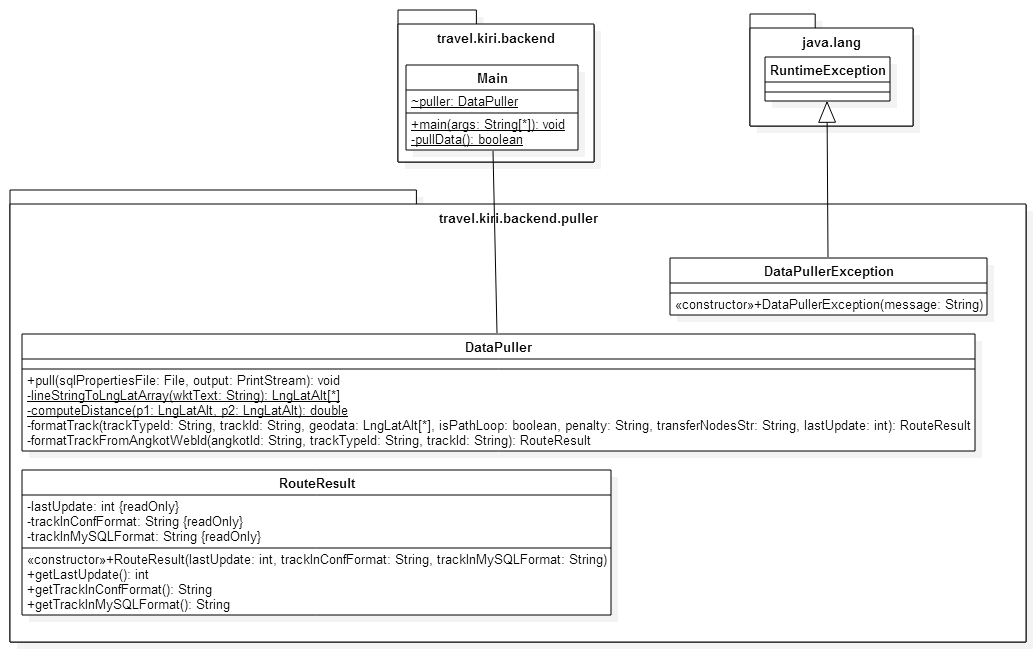
\includegraphics[scale=0.45]{Gambar/4_diagram_kelas}
	\caption{Diagram Kelas (Tahap Desain)} 
	\label{fig:4_diagram_kelas}
\end{figure}

\section{Perancangan Protokol}

Protokol untuk melakukan sinkronisasi dibuat di atas protokol \textit{Transportation List} dan \textit{Transportation Detail} milik situs Peta Angkutan Umum. Di awal sinkronisasi, mesin navigasi KIRI mencatat trayek apa saja yang harus disinkronkan dengan Peta Angkutan Umum. Kemudian, mesin navigasi KIRI akan mengirimkan permintaan \textit{Transportartion List} dengan menyertakan parameter id/kode angkot Peta Angkutan Umum, yang dipisahkan dengan \textit{pipe} ("|"). Tambahan parameter ini merupakan hasil dari optimasi protokol yang sudah ada, sehingga jawaban yang dikirimkan hanya mencakup angkot yang diperlukan oleh KIRI saja.

Contohnya, permintaan \textit{Transportation List} yang meminta status dari angkot dengan kode 1 dan 2 saja menggunakan perintah \texttt{GET /route/transportation-list.json?id=1|2}. Hasil dari permintaan tersebut akan menghasilkan kembalian kurang lebih seperti berikut:

\begin{lstlisting}
{
   "transportations":[
      {
         "city":"Jakarta",
         "id":1,
         "updated":"1381097188",
         "number":"M17",
         "province":"ID-JK",
         "company":"Mikrolet",
         "created":"1376493332",
         "destination":"Pasar Lenteng Agung",
         "origin":"Pasar Minggu",
         "hasRoute":true
      },
      {
         "city":"Jakarta",
         "id":2,
         "updated":"1379737743",
         "number":"S616",
         "province":"ID-JK",
         "company":"Kopaja",
         "created":"1376494541",
         "destination":"Cipedak",
         "origin":"Blok M",
         "hasRoute":true
      }
   ],
   "status":"ok",
   "provinces":[
      [
         "ID-AC",
         "Aceh"
      ],
      ...
    ]
}
\end{lstlisting}

Dari kembalian di atas, mesin navigasi KIRI dapat mengetahui kapan rute di Peta Angkutan Umum terakhir diperbaharui, untuk trayek-trayek yang diminta. Untuk setiap rute yang telah berubah, KIRI mengirimkan lagi perintah berikutnya, yaitu \textit{Transportation Detail}, yang memberikan rute penuh untuk trayek yang diminta. Sebagai contoh, jika rute dengan kode 1 ditemukan telah berubah, maka akan dikirimkan perintah \textit{Transportation Detail} \texttt{GET /route/transportation/1.json}. Dari situ, rute lengkap akan disimpan pada berkas \texttt{tracks.conf}.

\section{Perancangan Antarmuka}

\subsection{Antarmuka Mesin Navigasi KIRI}

Mesin navigasi KIRI adalah program yang dijalankan sebagai server, sehingga hanya memiliki antarmuka minimal berbasis teks yang menampilkan aksi-aksi yang dilakukan oleh server. Setelah ditambahkan fitur menarik data dari Peta Angkutan Umum, maka akan ada tambahan penampilan aksi menarik rute seperti contoh berikut (tambahan ada pada baris 1-8):

\begin{lstlisting}
May 20, 2015 1:56:02 PM travel.kiri.backend.puller.DataPuller pull
INFO: Fetching https://angkot.web.id/route/transportation-list.json?id=157|247|636...
May 20, 2015 1:56:11 PM travel.kiri.backend.puller.DataPuller formatTrackFromAngkotWebId
INFO: Fetching bdo_angkot.cicaheumciroyom from https://angkot.web.id/route/transportation/157.json...
May 20, 2015 1:56:17 PM travel.kiri.backend.puller.DataPuller formatTrackFromAngkotWebId
INFO: Fetching bdo_angkot.cicaheumledeng from https://angkot.web.id/route/transportation/247.json...
May 20, 2015 1:56:19 PM travel.kiri.backend.puller.DataPuller formatTrackFromAngkotWebId
INFO: Fetching bdo_angkot.ciroyomantapani from https://angkot.web.id/route/transportation/636.json...
May 20, 2015 1:56:37 PM travel.kiri.backend.Worker <init>
INFO: Configuration were read successfully
May 20, 2015 1:56:41 PM travel.kiri.backend.Worker <init>
INFO: Tracks were read successfully
May 20, 2015 1:57:04 PM travel.kiri.backend.Worker <init>
INFO: Tracks were linked successfully
2015-05-20 13:57:07.356:INFO::main: Logging initialized @65987ms
2015-05-20 13:57:10.173:INFO:oejs.Server:main: jetty-9.2.3.v20140905
2015-05-20 13:57:11.483:INFO:oejs.ServerConnector:main: Started ServerConnector@2996771e{HTTP/1.1}{0.0.0.0:8000}
2015-05-20 13:57:11.485:INFO:oejs.Server:main: Started @70398ms"
\end{lstlisting}


\subsection{Antarmuka Situs Web KIRI}

Pada situs web KIRI, jika ditemukan rute yang dihasilkan terintegrasi dengan Peta Angkutan Umum, maka situs akan menambahkan sebuah tombol kecil berbentuk pensil, yang jika diklik akan membawa pengguna ke situs Peta Angkutan Umum untuk memodifikasi rute terkait. Tampilan tombol tersebut dapat dilihat di gambar \ref{fig:4_tombolubah} (diberi panah merah).

\begin{figure}
	\centering
	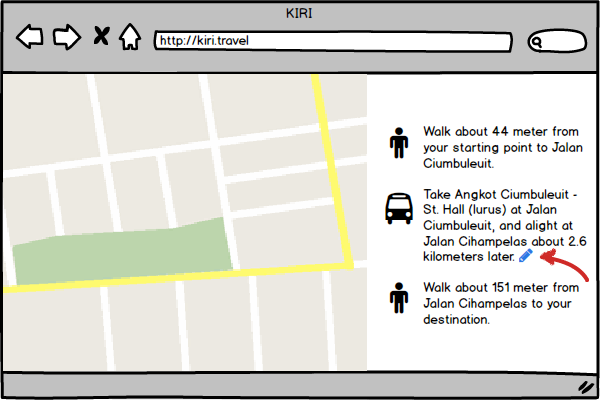
\includegraphics[scale=0.5]{Gambar/4_tombolubah}
	\caption{Tombol ubah di situs web KIRI} 
	\label{fig:4_tombolubah}
\end{figure}}{}
\ifdefstring{\vbabe}{1}{\chapter{Implementasi dan Pengujian}
\label{chap:implementasi_pengujian}

\section{Implementasi}

Implementasi dilakukan pada sebuah mesin virtual yang dibuat pada \textit{platform Windows Azure}. Mesin virtual ini terhubung ke internet serta beroperasi 24 jam sehingga dapat melayani permintaan tanpa henti. Adapun spesifikasi dari mesin virtual ini adalah sebagai berikut:

\begin{itemize}
	\item Prosesor: 1 core
	\item RAM: 1.75 GB
	\item Hard disk: 28.8 GB
	\item Sistem Operasi: Ubuntu 14.04.2 LTS (64-bit)
\end{itemize}

\section{Pengujian}

\subsection{Pengujian Fungsional}

TODO

\subsection{Pengujian Eksperimental}

Pengujian eksperimental dibagi menjadi 3 tahap:

\begin{enumerate}
	\item Survei \textit{online} terhadap kepuasan kualitas pencarian pengguna, dan potensi keinginan untuk berkontribusi selama satu bulan.
	\item Kampanye fitur integrasi perbaikan rute melalui Facebook selama satu bulan.
	\item Survei \textit{online} terhadap kepuasan kualitas pencarian serta keterlibatan pengguna dalam perbaikan rute.
\end{enumerate}

Ketiga tahap tersebut dijelaskan pada subbab-subbab berikut.

\subsubsection{Tahap 1: Survei Kepuasan Kualitas Pencarian dan Potensi Keinginan Berkontribusi}

Pada tahap ini, peneliti membuat survei \textit{online} memanfaatkan aplikasi Google Docs\footnote{\url{https://google.com/docs}}. Ada 6 pertanyaan yang ditanyakan, yaitu:

\begin{itemize}
	\item \textbf{Seberapa baik rute kami secara keseluruhan?} (mengerikan / buruk / netral / baik / sempurna)
	\item \textbf{Seberapa baik rute kami pada bagian rute kendaraan?} (mengerikan / buruk / netral / baik / sempurna)
	\item \textbf{Seberapa baik rute kami pada bagian rute berjalan?} (mengerikan / buruk / netral / baik / sempurna)
	\item \textbf{Di kota apa Anda menggunakan KIRI?} (Bandung / Jakarta / Malang / Surabaya)
	\item \textbf{Di mana Anda tinggal?} (Bandung / Jakarta / Malang / Surabaya)
	\item \textbf{Apakah Anda tertarik untuk berkontribusi data rute?} (Ya, dengan imbalan / Ya, tanpa syarat / Tidak / Tidak tahu)
\end{itemize}

Survei ini disediakan \textit{online} pada alamat \url{http://goo.gl/forms/WkeU8oK4Ek}, dan ditunjukkan pada situs web KIRI setelah hasil pencarian ditampilkan (Gambar TODO) selama bulan Mei 2015.

Setelah masa survei berakhir, didapatkan 33 responden survei. Dari segi kualitas pencarian (Gambar \ref{fig:5_hasilsurvei_1_1}), secara umum pengguna puas dengan hasil kualitas pencarian, ditandai dengan sebagian besar pengguna memilih "baik" pada ketiga jenis pertanyaan. Pada bagian kualitas rute kendaraan, relatif lebih banyak pengguna yang memilih "sempurna" dibandingkan dengan rute berjalan. Peneliti menduga bahwa ini dikarenakan oleh dua hal:

\begin{itemize}
	\item Pencarian rute di KIRI relatif lebih baik dibandingkan dengan pada situs web sejenis\footnote{\url{http://angkot.tibandung.com/}}, karena lebih presisi hingga titik koordinat.
	\item Karena keterbatasan data, hasil rute berjalan di KIRI menghasilkan garis lurus dan tidak mengikuti arah jalan yang sesungguhnya.
\end{itemize}

Dari segi demografi pengguna (\ref{fig:5_hasilsurvei_1_2}, sebagian besar pengguna menggunakan KIRI di Bandung dan tinggal di Bandung. Hal ini memberikan dua keuntungan kepada peneliti:

\begin{itemize}
	\item Sesuai dengan batasan masalah, yaitu penelitian dilakukan di kota Bandung.
	\item Pengguna relatif mengenal rute transportasi publik di Bandung, karena tinggal di kota Bandung.
\end{itemize}

Terakhir, survei mengenai potensi keinginan berkontribusi (\ref{fig:5_hasilsurvei_1_3}) memberikan hasil yang bervariasi. Sebagian besar responden bersedia memperbaiki rute yang salah, namun ada juga yang berharap imbalan maupun tidak berminat. Hasil tersebut cukup meyakinkan peneliti bahwa pada tahap berikutnya akan ada sebagian dari pengguna yang bersedia memperbaiki.

\begin{figure}
	\centering
	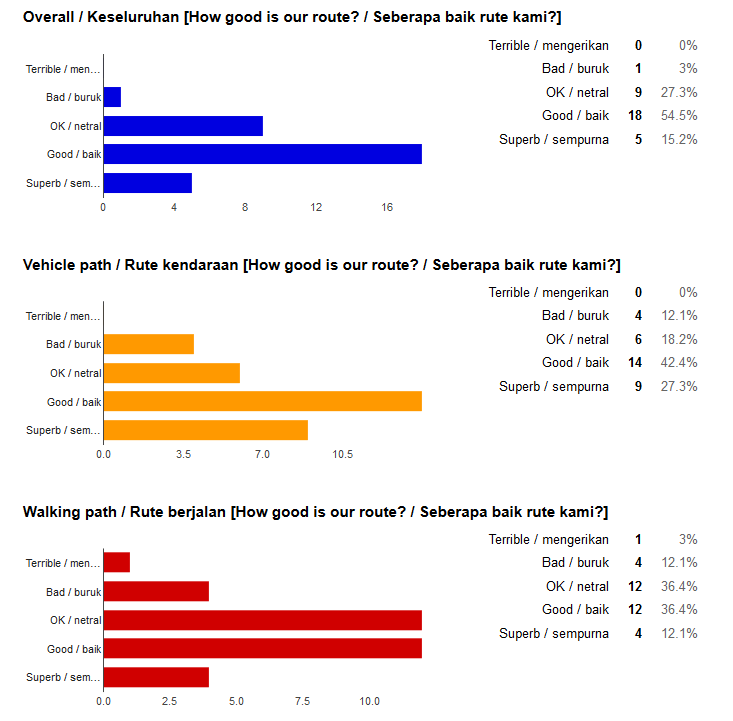
\includegraphics[scale=0.75]{Gambar/5_hasilsurvei_1_1}
	\caption{Hasil Survei Tahap 1 (Kualitas Pencarian)} 
	\label{fig:5_hasilsurvei_1_1}
\end{figure}

\begin{figure}
	\centering
	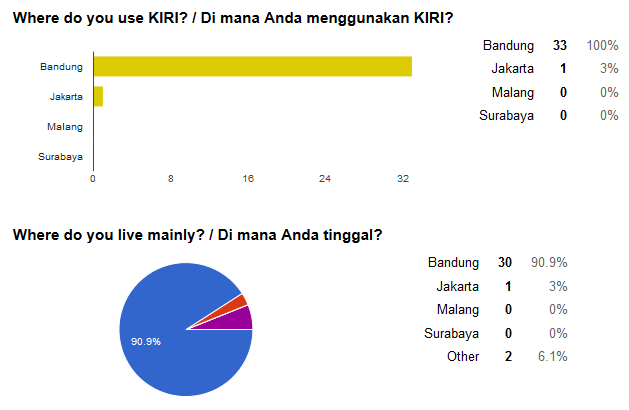
\includegraphics[scale=0.75]{Gambar/5_hasilsurvei_1_2}
	\caption{Hasil Survei Tahap 1 (Demografi Pengguna)} 
	\label{fig:5_hasilsurvei_1_2}
\end{figure}

\begin{figure}
	\centering
	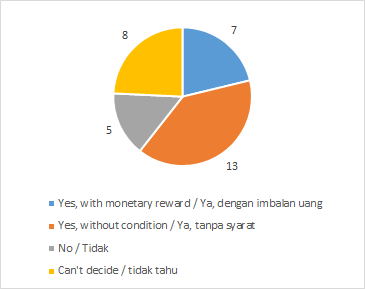
\includegraphics[scale=0.75]{Gambar/5_hasilsurvei_1_3}
	\caption{Hasil Survei Tahap 1 (Kesediaan Berkontribusi)} 
	\label{fig:5_hasilsurvei_1_3}
\end{figure}}{}
\ifdefstring{\vbabf}{1}{\chapter{Kesimpulan dan Saran}

\section{Kesimpulan}

Dari penelitian yang telah dilakukan, didapatkanlah kesimpulan-kesimpulan sebagai berikut:

\begin{enumerate}
	\item Telah berhasil diimplementasikan pengunduhan data otomatis oleh KIRI terhadap Peta Angkutan Umum secara berkala, setiap hari pukul 0.30. Pengunduhan data dilakukan dengan menggunakan \textit{HTTP Request} dan format data \textit{JSON} dan \textit{GeoJSON}.
	\item Telah berhasil diimplementasikan pemisahan data antara rute milik KIRI dengan data yang ditarik dari Peta Angkutan Umum. Dalam basis data KIRI, hal ini dicatat dalam kolom ``internalInfo'' dengan format ``angkotwebid:\textit{id-angkutan-umum}:\textit{waktu-terakhir-berubah}''.
	\item Protokol yang digunakan telah berhasil dioptimasi, dengan mencatat waktu terakhir sebuah rute diunduh. Dengan begitu, hanya rute yang berubah sejak pengunduhan terakhir saja yang diunduh kembali.
	\item Pengguna KIRI cukup puas dengan kualitas navigasi dari KIRI (mayoritas menjawab baik), dengan tingkat kepuasan rute kendaraan lebih tinggi dibanding rute berjalan. Pengguna KIRI masih belum berpartisipasi aktif dalam perbaikan rute.
\end{enumerate}

\section{Saran}

Dari hasil penelitian termasuk kesimpulan yang didapat, berikut adalah beberapa saran untuk pengembangan:

\begin{enumerate}
	\item Pada penelitian ini pengguna kurang berpartisipasi dalam perbaikan rute, sehingga sulit untuk menarik kesimpulan dari fitur sinkronisasi. Untuk pengembangan, disarankan untuk mengulang penelitian di kota yang lebih cocok: rute yang belum akurat, namun penduduknya memiliki semangat untuk berkontribusi.
	\item Penelitian ini memanfaatkan kolom ``internalInfo'' yang awalnya tidak didesain untuk menampung informasi penanda rute dari Peta Angkutan Umum. Dalam pengembangan perangkat lunak yang baik, ada baiknya penanda tersebut dipisahkan sehingga tidak mengganggu fungsi awal dari kolom ``internalInfo'' itu sendiri, yaitu menyimpan informasi yang dapat dimanfaatkan oleh administrator.
\end{enumerate}}{}
\ifdefstring{\vbabg}{1}{\include{Bab/bab7}}{}
\ifdefstring{\vbabh}{1}{\include{Bab/bab8}}{}
\ifdefstring{\vbabi}{1}{\include{Bab/bab9}}{}

\bibliographystyle{ieeetr}
\bibliography{pustaka}

\appendix
\apptoc

\tampillmp{\vlmp}
\ifdefstring{\vlmpa}{1}{\chapter{Kode Program Data Puller}

%selalu gunakan single spacing untuk source code !!!!!
\singlespacing 
% language: bahasa dari kode program
% terdapat beberapa pilihan : Java, C, C++, PHP, Matlab, R, dll
%
% basicstyle : ukuran font untuk kode program
% terdapat beberapa pilihan : tiny, scriptsize, footnotesize, dll
%
% caption : nama yang akan ditampilkan di dokumen akhir, lihat contoh
\begin{lstlisting}[language=Java,basicstyle=\tiny,caption=DataPuller.java]
package travel.kiri.backend.puller;

import java.io.File;
import java.io.FileReader;
import java.io.IOException;
import java.io.PrintStream;
import java.net.URL;
import java.sql.Connection;
import java.sql.DriverManager;
import java.sql.ResultSet;
import java.sql.SQLException;
import java.sql.Statement;
import java.util.ArrayList;
import java.util.List;
import java.util.Properties;
import java.util.SortedMap;
import java.util.TreeMap;

import org.geojson.Feature;
import org.geojson.LngLatAlt;
import org.geojson.MultiLineString;

import travel.kiri.backend.Main;

import com.fasterxml.jackson.core.JsonFactory;
import com.fasterxml.jackson.core.JsonParser;
import com.fasterxml.jackson.core.JsonToken;
import com.fasterxml.jackson.databind.JsonNode;
import com.fasterxml.jackson.databind.ObjectMapper;

public class DataPuller {
	public static final double EARTH_RADIUS = 6371.0;
	public static final Double MAX_DISTANCE = 0.1;
	public static final String ANGKOTWEBID_URL = "https://angkot.web.id/route/transportation/%s.json";
	public static final String ANGKOTWEBID_ROUTELIST_PREFIX = "https://angkot.web.id/route/transportation-list.json?id=";
	public static final int ANGKOTWEBID_MAX_ROUTELIST = 200;
	public static final String DEFAULT_PENALTY = "0.05";
	public static final double MAX_LINK_DISTANCE = 0.5;

	public void pull(File sqlPropertiesFile, PrintStream output)
			throws IOException, SQLException {
		Properties sqlProperties = new Properties();
		sqlProperties.load(new FileReader(sqlPropertiesFile));
		Connection connection = null;
		connection = DriverManager.getConnection(String.format(
				"jdbc:mysql://%s/%s?user=%s&password=%s",
				sqlProperties.get("host"), sqlProperties.get("database"),
				sqlProperties.get("user"), sqlProperties.get("password")));
		
		// Look for angkot.web.id refreshes
		Statement statement = connection.createStatement();
		ResultSet result = statement.executeQuery("SELECT trackTypeId, trackId, AsText(geodata), internalInfo FROM tracks");
		SortedMap<Integer, AngkotWebIdCacheInfo> obsoleteRoutesMap = new TreeMap<Integer, AngkotWebIdCacheInfo>();
		while (result.next()) {
			if (result.getString(4).startsWith("angkotwebid:")) {
				String[] fields = result.getString(4).split(":");
				int id = Integer.parseInt(fields[1]);
				long lastUpdate = fields.length > 2 ? Long.parseLong(fields[2]) : 0;
				obsoleteRoutesMap.put(id, new AngkotWebIdCacheInfo(result.getString(1), result.getString(2), lastUpdate, id, result.getString(3) != null));
			}
		}
		List<Integer> obsoleteRoutesList = new ArrayList<Integer>(obsoleteRoutesMap.keySet());
		for (int i = 0; i < (obsoleteRoutesList.size() + ANGKOTWEBID_MAX_ROUTELIST - 1) / ANGKOTWEBID_MAX_ROUTELIST; i++) {
			StringBuilder urlBuilder = new StringBuilder(ANGKOTWEBID_ROUTELIST_PREFIX);
			for (int j = i * 250; j < Math.min((i + 1) * 250, obsoleteRoutesList.size()); j++) {
				urlBuilder.append(j > i * 250 ? "|" : "");
				urlBuilder.append(obsoleteRoutesList.get(j));
			}
			Main.globalLogger.info("Fetching " + urlBuilder + "...");
			ObjectMapper mapper = new ObjectMapper();
			JsonNode parent = mapper.readTree(new URL(urlBuilder.toString()));
			JsonNode transportations = parent.get("transportations");
			for (int j = 0; j < transportations.size(); j++) {
				JsonNode transportation = transportations.get(j);
				int updated = transportation.get("updated").asInt();
				int id = transportation.get("id").asInt();
				if (obsoleteRoutesMap.get(id).pathAvailable && obsoleteRoutesMap.get(id).lastUpdate >= updated) {
					obsoleteRoutesMap.remove(id);
				}
			}
		}
		
		statement = connection.createStatement();
		result = statement
				.executeQuery("SELECT trackTypeId, trackId, AsText(geodata), pathloop, penalty, transferNodes, internalInfo FROM tracks ORDER BY trackTypeId, trackId");

		while (result.next()) {
			RouteResult routeResult;
			if (result.getString(7) != null
					&& result.getString(7).startsWith("angkotwebid:")) {
				String[] fields = result.getString(7).split(":");
				if (obsoleteRoutesMap.containsKey(Integer.parseInt(fields[1]))) {
					routeResult = formatTrackFromAngkotWebId(
							fields[1], result.getString(1), result.getString(2));
					if (routeResult != null) {
						Statement updateStatement = connection.createStatement();
						String sql = String
								.format("UPDATE tracks SET internalInfo='%s', geodata=%s WHERE trackTypeId='%s' AND trackId='%s'",
										fields[0] + ':' + fields[1]
												+ ':' + routeResult.lastUpdate,
										routeResult.getTrackInMySQLFormat(),
										result.getString(1),
										result.getString(2));
						updateStatement
								.execute(sql);
					}					
				} else {
					routeResult = formatTrack(result.getString(1), result
							.getString(2), lineStringToLngLatArray(result
							.getString(3)), result.getString(4).equals("1") ? true
							: false, result.getString(5), result.getString(6), 0);
				}
				output.println(routeResult.getTrackInConfFormat());
			} else if (result.getString(3) != null) {
				routeResult = formatTrack(result.getString(1), result
						.getString(2), lineStringToLngLatArray(result
						.getString(3)), result.getString(4).equals("1") ? true
						: false, result.getString(5), result.getString(6), 0);
				output.println(routeResult.getTrackInConfFormat());
			} else {
				throw new DataPullerException("Route not found everywhere for "
						+ result.getString(1) + "." + result.getString(2));
			}
		}

		result.close();
		statement.close();
		connection.close();
	}

	private static LngLatAlt[] lineStringToLngLatArray(String wktText) {
		wktText = wktText.replace("LINESTRING(", "").replace(")", "");
		String[] textCoordinates = wktText.split(",");
		LngLatAlt[] coordinates = new LngLatAlt[textCoordinates.length];
		for (int i = 0; i < textCoordinates.length; i++) {
			String[] textLonlat = textCoordinates[i].split(" ");
			LngLatAlt coordinate = new LngLatAlt(
					Double.parseDouble(textLonlat[0]),
					Double.parseDouble(textLonlat[1]));
			coordinates[i] = coordinate;
		}
		return coordinates;
	}

	private static double computeDistance(LngLatAlt p1, LngLatAlt p2) {
		double lat1 = p1.getLatitude(), lon1 = p1.getLongitude();
		double lat2 = p2.getLatitude(), lon2 = p2.getLongitude();
		double dLat = Math.toRadians(lat2 - lat1);
		double dLon = Math.toRadians(lon2 - lon1);
		lat1 = Math.toRadians(lat1);
		lat2 = Math.toRadians(lat2);
		double a = Math.sin(dLat / 2) * Math.sin(dLat / 2) + Math.sin(dLon / 2)
				* Math.sin(dLon / 2) * Math.cos(lat1) * Math.cos(lat2);
		double c = 2 * Math.atan2(Math.sqrt(a), Math.sqrt(1 - a));
		return EARTH_RADIUS * c;
	}

	private RouteResult formatTrack(String trackTypeId, String trackId,
			LngLatAlt[] geodata, boolean isPathLoop, String penalty,
			String transferNodesStr, int lastUpdate) {

		// Setup track info
		LngLatAlt[] tracks = geodata;
		int[][] transitNodes;
		if (transferNodesStr == null || transferNodesStr.length() == 0) {
			transitNodes = new int[][] { { 0, tracks.length - 1 } };
		} else {
			String[] transitNodesString = transferNodesStr.split(",");
			transitNodes = new int[transitNodesString.length][2];
			for (int i = 0; i < transitNodes.length; i++) {
				String[] numbers = transitNodesString[i].split("-");
				transitNodes[i][0] = Integer.parseInt(numbers[0]);
				transitNodes[i][1] = Integer
						.parseInt(numbers.length > 1 ? numbers[1] : numbers[0]);
			}
		}

		List<LngLatAlt> trackString = new ArrayList<LngLatAlt>();

		int insertedNodes = 0;
		int[] transferNodesOffset = new int[tracks.length];
		LngLatAlt previousPoint = null;

		// Print tracks
		for (int i = 0; i < tracks.length; i++) {
			LngLatAlt currentPoint = tracks[i];
			if (i > 0) {
				boolean inTransitNode = false;
				for (int j = 0; j < transitNodes.length; j++) {
					if (i >= transitNodes[j][0] && i <= transitNodes[j][1]) {
						inTransitNode = true;
					}
				}
				// then, check if we have to add virtual nodes
				double distance;
				if (MAX_DISTANCE != null
						&& (distance = computeDistance(currentPoint,
								previousPoint)) > MAX_DISTANCE && inTransitNode) {
					int extraNodes = (int) Math.ceil(distance / MAX_DISTANCE) - 1;
					for (int j = 1; j <= extraNodes; j++) {
						double lat = previousPoint.getLatitude()
								+ j
								* (currentPoint.getLatitude() - previousPoint
										.getLatitude()) / extraNodes;
						double lng = previousPoint.getLongitude()
								+ j
								* (currentPoint.getLongitude() - previousPoint
										.getLongitude()) / extraNodes;
						LngLatAlt extraPoint = new LngLatAlt(lng, lat);
						trackString.add(extraPoint);
					}
					insertedNodes += extraNodes;
				}
			}
			transferNodesOffset[i] = insertedNodes;
			trackString.add(currentPoint);
			previousPoint = currentPoint;
		}

		for (int i = 0; i < transitNodes.length; i++) {
			// Adjust with offset
			for (int j = 0; j < 2; j++) {
				transitNodes[i][j] += transferNodesOffset[transitNodes[i][j]];
			}
		}
		StringBuilder finalTextConf = new StringBuilder();
		StringBuilder finalTextMySQL = new StringBuilder("GeomFromText('LineString(");
		finalTextConf.append(trackTypeId + "." + trackId + "\t");
		finalTextConf.append(penalty + "\t");
		finalTextConf.append(trackString.size() + "\t");
		for (int i = 0; i < trackString.size(); i++) {
			if (i > 0) {
				finalTextConf.append(" ");
				finalTextMySQL.append(",");
			}
			finalTextConf.append(String.format("%.6f %.6f", trackString.get(i)
					.getLatitude(), trackString.get(i).getLongitude()));
			finalTextMySQL.append(String.format("%.6f %.6f", trackString.get(i)
					.getLongitude(), trackString.get(i).getLatitude()));
		}
		finalTextConf.append("\t");
		finalTextConf.append((isPathLoop ? "1" : "0") + "\t");
		for (int i = 0; i < transitNodes.length; i++) {
			if (i > 0) {
				finalTextConf.append(",");
			}
			if (transitNodes[i][0] == transitNodes[i][1]) {
				finalTextConf.append(transitNodes[i][0]);
			} else {
				finalTextConf.append(String.format("%d-%d", transitNodes[i][0],
						transitNodes[i][1]));
			}
		}
		finalTextMySQL.append(")')");
		return new RouteResult(lastUpdate, finalTextConf.toString(), finalTextMySQL.toString());
	}

	private RouteResult formatTrackFromAngkotWebId(String angkotId,
			String trackTypeId, String trackId) throws IOException {
		URL url = new URL(String.format(ANGKOTWEBID_URL, angkotId));
		Main.globalLogger.info("Fetching " + trackTypeId + "." + trackId
				+ " from " + url + "...");
		JsonFactory factory = new JsonFactory();
		JsonParser parser = factory.createParser(url);

		List<LngLatAlt> finalCoordinates = null;
		Boolean isPathLoop = null;
		int lastUpdate = -1;
		while (!parser.isClosed()) {
			JsonToken token = parser.nextToken();
			if (token == null) {
				break;
			}
			if (JsonToken.FIELD_NAME.equals(token)
					&& "updated".equals(parser.getCurrentName())) {
				parser.nextValue();
				lastUpdate = parser.getValueAsInt();
			} else if (JsonToken.FIELD_NAME.equals(token)
					&& "geojson".equals(parser.getCurrentName())) {
				parser.nextBooleanValue();
				Feature feature = new ObjectMapper().readValue(parser,
						Feature.class);
				List<List<LngLatAlt>> coordinates = ((MultiLineString) feature
						.getGeometry()).getCoordinates();
				if (coordinates.size() == 0) {
					Main.globalLogger.warning(String.format(
							"%s.%s/%s has zero routes, will be ignored.",
							trackTypeId, trackId, angkotId));
					return null;
				}
				if (coordinates.size() == 1) {
					finalCoordinates = coordinates.get(0);
					isPathLoop = computeDistance(finalCoordinates.get(0),
							finalCoordinates.get(finalCoordinates.size() - 1)) < MAX_LINK_DISTANCE;
				} else if (coordinates.size() == 2) {
					List<LngLatAlt> c1 = coordinates.get(0);
					List<LngLatAlt> c2 = coordinates.get(1);
					if (computeDistance(c1.get(c1.size() - 1), c2.get(0)) < MAX_LINK_DISTANCE
							&& computeDistance(c1.get(0), c2.get(c2.size() - 1)) < MAX_LINK_DISTANCE) {
						finalCoordinates = c1;
						finalCoordinates.addAll(c2);
						isPathLoop = true;
					} else if (computeDistance(c1.get(0), c2.get(0)) < MAX_LINK_DISTANCE
							&& computeDistance(c1.get(c1.size() - 1),
									c2.get(c2.size() - 1)) < MAX_LINK_DISTANCE) {
						finalCoordinates = c1;
						for (int j = c2.size() - 1; j >= 0; j--) {
							finalCoordinates.add(c2.get(j));
						}
						isPathLoop = true;
					} else {
						throw new DataPullerException(
								String.format(
										"Does not support linking tracks that far away: %s.%s/%s ",
										trackTypeId, trackId, angkotId));
					}
				} else {
					Main.globalLogger
							.warning(String
									.format("Does not support tracks with %d routes: %s.%s/%s ",
											coordinates.size(), trackTypeId,
											trackId, angkotId));
					return null;
				}
			}
		}
		if (finalCoordinates != null) {
			RouteResult result = formatTrack(trackTypeId, trackId,
					finalCoordinates.toArray(new LngLatAlt[0]), isPathLoop,
					DEFAULT_PENALTY, null, lastUpdate);
			return result;
		} else {
			Main.globalLogger.warning("Doesn't have GeoJSON info: " + angkotId);
			return null;
		}
	}

	public static class RouteResult {
		private final int lastUpdate;
		private final String trackInConfFormat;
		private final String trackInMySQLFormat;

		public RouteResult(int lastUpdate, String trackInConfFormat,
				String trackInMySQLFormat) {
			super();
			this.lastUpdate = lastUpdate;
			this.trackInConfFormat = trackInConfFormat;
			this.trackInMySQLFormat = trackInMySQLFormat;
		}

		public int getLastUpdate() {
			return lastUpdate;
		}

		public String getTrackInConfFormat() {
			return trackInConfFormat;
		}

		public String getTrackInMySQLFormat() {
			return trackInMySQLFormat;
		}

	}
	
	private static class AngkotWebIdCacheInfo {
		public final long lastUpdate;
		public final boolean pathAvailable;
		
		public AngkotWebIdCacheInfo(String trackTypeId, String trackId,
				long lastUpdate, int id, boolean pathAvailable) {
			super();
			this.lastUpdate = lastUpdate;
			this.pathAvailable = pathAvailable;
		}
		
		
	}
}
\end{lstlisting}

%selalu gunakan single spacing untuk source code !!!!!
\singlespacing 
% language: bahasa dari kode program
% terdapat beberapa pilihan : Java, C, C++, PHP, Matlab, R, dll
%
% basicstyle : ukuran font untuk kode program
% terdapat beberapa pilihan : tiny, scriptsize, footnotesize, dll
%
% caption : nama yang akan ditampilkan di dokumen akhir, lihat contoh
\begin{lstlisting}[language=Java,basicstyle=\tiny,caption=DataPullerException.java]
package travel.kiri.backend.puller;

public class DataPullerException extends RuntimeException {

	private static final long serialVersionUID = -5734202145456381699L;

	public DataPullerException(String message) {
		super(message);
	}
}
\end{lstlisting}}{}
\ifdefstring{\vlmpb}{1}{\chapter{The Source Code}
\label{app:B}

%selalu gunakan single spacing untuk source code !!!!!
\singlespacing 
% language: bahasa dari kode program
% terdapat beberapa pilihan : Java, C, C++, PHP, Matlab, R, dll
%
% basicstyle : ukuran font untuk kode program
% terdapat beberapa pilihan : tiny, scriptsize, footnotesize, dll
%
% caption : nama yang akan ditampilkan di dokumen akhir, lihat contoh
\begin{lstlisting}[language=Java,basicstyle=\tiny,caption=MainActivity.java]
package com.example.egaprianto.testingsensors;

import android.content.Intent;
import android.hardware.Sensor;
import android.hardware.SensorManager;
import android.support.v7.app.AppCompatActivity;
import android.os.Bundle;
import android.view.View;
import android.widget.TextView;

public class MainActivity extends AppCompatActivity {
    TextView mTextView; 
    private SensorManager mSensorManager;
    private Sensor mSensor;

    @Override
    protected void onCreate(Bundle savedInstanceState) {
        super.onCreate(savedInstanceState);
        setContentView(R.layout.activity_main);
    }

    @Override
    public void onDestroy() {
        super.onDestroy();
        android.os.Debug.stopMethodTracing();
    }

    public void onClickLightSensorButton(View view){
        Intent intent = new Intent(this, SensorAccelerometerActivity.class);
        startActivity(intent);
    }

    public void onRotVecSensorButton(View view){
        Intent intent = new Intent(this, QuaternionTheta.class);
        startActivity(intent);
    }

    public void recordAllRAWSensorData(View view){
        Intent intent = new Intent(this, RecordAllRAWSensorData.class);
        startActivity(intent);
    }

    public void onGyroSensorClicked(View view){
        Intent intent = new Intent(this, SensorGyroscopeActivity.class);
        startActivity(intent);
    }
    public void onMagSensorClicked(View view){
        Intent intent = new Intent(this, SensorGeomagnetoticRotationActivity.class);
        startActivity(intent);
    }
}

\end{lstlisting}
\begin{lstlisting}[language=Java,basicstyle=\tiny,caption=RecordAllRAWSensorData.java]
package com.example.egaprianto.testingsensors;

import android.Manifest;
import android.content.Context;
import android.content.pm.PackageManager;
import android.hardware.Sensor;
import android.hardware.SensorEvent;
import android.hardware.SensorEventListener;
import android.hardware.SensorManager;
import android.media.Ringtone;
import android.media.RingtoneManager;
import android.net.Uri;
import android.os.Build;
import android.os.Bundle;
import android.os.CountDownTimer;
import android.os.Environment;
import android.support.v4.app.ActivityCompat;
import android.support.v7.app.AppCompatActivity;
import android.text.format.DateFormat;
import android.util.Log;
import android.view.View;
import android.view.WindowManager;
import android.widget.TextView;


import java.io.BufferedWriter;
import java.io.File;
import java.io.FileWriter;
import java.io.IOException;
import java.util.ArrayList;
import java.util.List;

public class RecordAllRAWSensorData extends AppCompatActivity implements SensorEventListener {
    private static final String FILENAME = "sensorRecord-";
    private SensorManager mSensorManager;
    private ArrayList<Sensor> sensorArrayList;
    private TextView textViewCountDown;
    private boolean isCapturing;
    private File file;
    private ArrayList<double[]> acceleroData;
    private ArrayList<double[]> gyroData;
    private long startCaptureTime;
    private long runningTime;
    private ArrayList<double[]> rotData;
    private ArrayList<double[]> rotVecData;

    @Override
    protected void onCreate(Bundle savedInstanceState) {
        super.onCreate(savedInstanceState);
        this.sensorArrayList = new ArrayList<Sensor>();
        setContentView(R.layout.activity_record_all_rawsensor_data);
        mSensorManager = (SensorManager) getSystemService(Context.SENSOR_SERVICE);
        textViewCountDown = (TextView) findViewById(R.id.textViewCountDown);
        if (Build.VERSION.SDK_INT >= Build.VERSION_CODES.ICE_CREAM_SANDWICH_MR1) {
            this.sensorArrayList.add(sensorGetter(Sensor.TYPE_ACCELEROMETER));
            this.sensorArrayList.add(sensorGetter(Sensor.TYPE_GYROSCOPE));
            this.sensorArrayList.add(sensorGetter(Sensor.TYPE_ROTATION_VECTOR));
        }

        int REQUEST_EXTERNAL_STORAGE = 1;
        String[] PERMISSIONS_STORAGE = {
                Manifest.permission.READ_EXTERNAL_STORAGE,
                Manifest.permission.WRITE_EXTERNAL_STORAGE
        };
        int permission = ActivityCompat.checkSelfPermission(this, Manifest.permission.WRITE_EXTERNAL_STORAGE);
        if (permission != PackageManager.PERMISSION_GRANTED) {
            ActivityCompat.requestPermissions(
                    this,
                    PERMISSIONS_STORAGE,
                    REQUEST_EXTERNAL_STORAGE
            );
        }
        isCapturing = false;
        for (Sensor sensor :
                sensorArrayList) {
            mSensorManager.registerListener(this, sensor, SensorManager.SENSOR_DELAY_GAME);
        }
    }

    @Override
    protected void onResume() {
        super.onResume();
        for (Sensor sensor :
                sensorArrayList) {
            mSensorManager.registerListener(this, sensor, SensorManager.SENSOR_DELAY_GAME);
        }
    }

    @Override
    protected void onPause() {
        super.onPause();
        mSensorManager.unregisterListener(this);
    }

    @Override
    public void onSensorChanged(SensorEvent event) {
        Sensor sensor = event.sensor;
        if (isCapturing) {
            float[] copyData = new float[4];
            System.arraycopy(event.values, 0, copyData, 1, 3);
            copyData[0] = System.currentTimeMillis() - startCaptureTime;
            if (sensor.getType() == Sensor.TYPE_ACCELEROMETER) {
                this.acceleroData.add(convertFloatsToDoubles(copyData));
            } else if (sensor.getType() == Sensor.TYPE_GYROSCOPE) {
                this.gyroData.add(convertFloatsToDoubles(copyData));
            }else if (sensor.getType() == Sensor.TYPE_ROTATION_VECTOR) {
                copyData = new float[6];
                System.arraycopy(event.values, 0, copyData, 1, event.values.length);
                copyData[0] = System.currentTimeMillis() - startCaptureTime;
                this.rotData.add(convertFloatsToDoubles(copyData));
                double theta = (Math.acos(event.values[3]))*2;
                double x = event.values[0]/ Math.sin(theta/2);
                double y = event.values[1]/ Math.sin(theta/2);
                double z = event.values[2]/ Math.sin(theta/2);
                double [] vecData = new double[5];
                vecData[0] = copyData[0];
                vecData[1] = x;
                vecData[2] = y;
                vecData[3] = z;
                vecData[4] = theta;
                this.rotVecData.add(vecData);
            }
            runningTime = (System.currentTimeMillis() - startCaptureTime);
            this.textViewCountDown.setText("Time : " + runningTime / 1000 + "sec");
        }
    }

    @Override
    public void onAccuracyChanged(Sensor sensor, int accuracy) {

    }

    public void onStartButtonClicked(View view) throws InterruptedException {
        Uri notification = RingtoneManager.getDefaultUri(RingtoneManager.TYPE_NOTIFICATION);
        Ringtone r = RingtoneManager.getRingtone(getApplicationContext(), notification);
        acceleroData = new ArrayList<double[]>();
        gyroData = new ArrayList<double[]>();
        rotData = new ArrayList<double[]>();
        rotVecData = new ArrayList<double[]>();
        String time = DateFormat.format("MM-dd-yyyyy-h|mm|ss-aa", System.currentTimeMillis()).toString();
        File root = new File(Environment.getExternalStoragePublicDirectory(Environment.DIRECTORY_DOCUMENTS) + File.separator + "DataSensors");
        root.mkdirs();
        file = new File(root, FILENAME + time + ".csv");
        try {
            file.createNewFile();
        } catch (IOException e) {
            e.printStackTrace();
        }
        new CountDownTimer(10000, 1000) {

            public void onTick(long millisUntilFinished) {
                textViewCountDown.setText("Count Down = " + millisUntilFinished / 1000);
            }

            public void onFinish() {
                textViewCountDown.setText("Capturing Data!");
                Uri notification = RingtoneManager.getDefaultUri(RingtoneManager.TYPE_NOTIFICATION);
                Ringtone r = RingtoneManager.getRingtone(getApplicationContext(), notification);
                r.play();
                isCapturing = true;
                getWindow().addFlags(WindowManager.LayoutParams.FLAG_KEEP_SCREEN_ON);
                startCaptureTime = System.currentTimeMillis();
            }
        }.start();

    }

    private Sensor sensorGetter(int input) {

        List<Sensor> sensorList = mSensorManager.getSensorList(input);
        Sensor sensor = null;
        for (int i = 0; i < sensorList.size(); i++) {
            sensor = sensorList.get(i);
        }
        return sensor;
    }

    private void writeData(BufferedWriter bw, ArrayList<double[]> data, String title, String columnTitle) throws IOException {
        bw.write(title);
        bw.newLine();
        bw.write(columnTitle);
        bw.newLine();
        for (int i = 0; i < data.size(); i++) {
            for (int j = 0; j < data.get(i).length; j++) {
                bw.write(data.get(i)[j] + ",");
            }
            bw.newLine();
        }
        bw.newLine();
    }

    private double[] convertFloatsToDoubles(float[] input)
    {
        if (input == null)
        {
            return null;
        }
        double[] output = new double[input.length];
        for (int i = 0; i < input.length; i++)
        {
            output[i] = input[i];
        }
        return output;
    }

    public void onStopButtonClicked(View view) {
        isCapturing = false;
        getWindow().clearFlags(WindowManager.LayoutParams.FLAG_KEEP_SCREEN_ON);
        try {
            BufferedWriter bw = new BufferedWriter(new FileWriter(this.file));
            writeData(bw, acceleroData, "Accelerometer", "time,x,y,z");
            writeData(bw, gyroData, "Gyroscope", "time,x,y,z");
            writeData(bw, rotData, "Rotation Vector", "time,x*sin(theta/2),y*sin(theta/2),z*sin(theta/2),cos(theta/2),akurasi (dalam radians) (-1 jika tidak ada)");
            writeData(bw, rotVecData, "Rotation Vector by Vector and Angle", "time,x,y,z,theta");
            bw.newLine();
            bw.write("Running Time : " + runningTime + "ms");
            bw.flush();
            bw.close();
            file.createNewFile();
            textViewCountDown.setText("Data Captured! at " + file.getAbsolutePath());
            Log.d("File", "File is located at " + file.getAbsolutePath());
        } catch (IOException e) {
            e.printStackTrace();
        }

    }
}

\end{lstlisting}
\begin{lstlisting}[language=Java,basicstyle=\tiny,caption=SensorAccelerometerActivity.java]
package com.example.egaprianto.testingsensors;

import android.app.Activity;
import android.content.Context;
import android.hardware.Sensor;
import android.hardware.SensorEvent;
import android.hardware.SensorEventListener;
import android.hardware.SensorManager;
import android.os.Build;
import android.os.Bundle;
import android.widget.TextView;

import java.util.List;

public class SensorAccelerometerActivity extends Activity implements SensorEventListener {
    private SensorManager mSensorManager;
    private Sensor mAccelSensor;
    private TextView textViewXData;
    private TextView textViewYData;
    private TextView textViewZData;
    private TextView textViewDebug;
    private TextView textViewAccuracy;

    @Override
    public final void onCreate(Bundle savedInstanceState) {
        super.onCreate(savedInstanceState);
        setContentView(R.layout.activity_accelero_sensor);
        textViewXData = (TextView) findViewById(R.id.textViewXData);
        textViewYData = (TextView) findViewById(R.id.textViewYData);
        textViewZData = (TextView) findViewById(R.id.textViewZData);
        textViewDebug = (TextView) findViewById(R.id.textViewDebug);
        textViewAccuracy = (TextView) findViewById(R.id.textViewAccuracy);
        mSensorManager = (SensorManager) getSystemService(Context.SENSOR_SERVICE);
        if (Build.VERSION.SDK_INT >= Build.VERSION_CODES.ICE_CREAM_SANDWICH_MR1) {
            mSensorManager = (SensorManager) getSystemService(Context.SENSOR_SERVICE);
            List<Sensor> accelerometerSensors = mSensorManager.getSensorList(Sensor.TYPE_ACCELEROMETER);
            mAccelSensor = null;
            if (accelerometerSensors != null) {
                for (int i = 0; i < accelerometerSensors.size(); i++) {
                    mAccelSensor = accelerometerSensors.get(i);
                }
            }
        }
    }

    @Override
    public final void onAccuracyChanged(Sensor sensor, int accuracy) {
    }

    @Override
    public final void onSensorChanged(SensorEvent event) {
        float x = event.values[0];
        float y = event.values[1];
        float z = event.values[2];
        textViewXData.setText("x = " + x);
        textViewYData.setText("y = " + y);
        textViewZData.setText("z = " + z);
    }

    @Override
    protected void onResume() {
        super.onResume();
        mSensorManager.registerListener(this, mAccelSensor, SensorManager.SENSOR_DELAY_NORMAL);
    }

    @Override
    protected void onPause() {
        super.onPause();
        mSensorManager.unregisterListener(this);
    }


}
\end{lstlisting}
\begin{lstlisting}[language=Java,basicstyle=\tiny,caption=SensorGyroscopeActivity.java]
package com.example.egaprianto.testingsensors;

import android.app.Activity;
import android.content.Context;
import android.hardware.Sensor;
import android.hardware.SensorEvent;
import android.hardware.SensorEventListener;
import android.hardware.SensorManager;
import android.os.Build;
import android.os.Bundle;
import android.widget.TextView;

import java.util.List;

public class SensorGyroscopeActivity extends Activity implements SensorEventListener {
    private SensorManager mSensorManager;
    private Sensor mGryoSensor;
    private TextView textViewXData;
    private TextView textViewYData;
    private TextView textViewZData;
    private TextView textViewDebug;
    private TextView textViewAccuracy;

    @Override
    public final void onCreate(Bundle savedInstanceState) {
        super.onCreate(savedInstanceState);
        setContentView(R.layout.activity_gyroscope_sensor);
        textViewXData = (TextView) findViewById(R.id.textViewXData);
        textViewYData = (TextView) findViewById(R.id.textViewYData);
        textViewZData = (TextView) findViewById(R.id.textViewZData);
        textViewDebug = (TextView) findViewById(R.id.textViewDebug);
        textViewAccuracy = (TextView) findViewById(R.id.textViewAccuracy);
        mSensorManager = (SensorManager) getSystemService(Context.SENSOR_SERVICE);
        if (Build.VERSION.SDK_INT >= Build.VERSION_CODES.ICE_CREAM_SANDWICH_MR1) {
            mSensorManager = (SensorManager) getSystemService(Context.SENSOR_SERVICE);
            List<Sensor> gyroscopeSensors = mSensorManager.getSensorList(Sensor.TYPE_GYROSCOPE);
            mGryoSensor = null;
            if (gyroscopeSensors != null) {
                for (int i = 0; i < gyroscopeSensors.size(); i++) {
                    mGryoSensor = gyroscopeSensors.get(i);
                }
            }
        }
    }

    @Override
    public final void onAccuracyChanged(Sensor sensor, int accuracy) {
    }

    @Override
    public final void onSensorChanged(SensorEvent event) {
        float x = event.values[0];
        float y = event.values[1];
        float z = event.values[2];
        textViewXData.setText("x = " + x);
        textViewYData.setText("y = " + y);
        textViewZData.setText("z = " + z);
    }

    @Override
    protected void onResume() {
        super.onResume();
        mSensorManager.registerListener(this, mGryoSensor, SensorManager.SENSOR_DELAY_NORMAL);
    }

    @Override
    protected void onPause() {
        super.onPause();
        mSensorManager.unregisterListener(this);
    }


}
\end{lstlisting}}{}
\ifdefstring{\vlmpc}{1}{\include{Lampiran/lampC}}{}
\ifdefstring{\vlmpd}{1}{\include{Lampiran/lampD}}{}
\ifdefstring{\vlmpe}{1}{\include{Lampiran/lampE}}{}
\ifdefstring{\vlmpf}{1}{\include{Lampiran/lampF}}{}
\ifdefstring{\vlmpg}{1}{\include{Lampiran/lampG}}{}
\ifdefstring{\vlmph}{1}{\include{Lampiran/lampH}}{}
\ifdefstring{\vlmpi}{1}{\include{Lampiran/lampI}}{}

\end{document}
